% !TeX program = xelatex
% !TeX encoding = UTF-8
\documentclass[a4paper,reqno,oneside]{book}

% ==================== XeLaTeX / Unicode ====================
\usepackage{fontspec}
\usepackage{polyglossia}
\setdefaultlanguage{vietnamese}
\setmainfont{Times New Roman}
\setsansfont{Arial}
\setmonofont{Consolas}
\usepackage{scrextend}
\changefontsizes{13pt}

% ==================== Gói dùng chung ====================
\usepackage{amsmath,amssymb,mathtools,amsfonts}
\usepackage{graphicx}
\usepackage{booktabs,longtable,array,tabularx,multirow}
\usepackage{float}
\usepackage{placeins}
\usepackage[table]{xcolor}
\usepackage{enumitem}
\usepackage{caption}
\usepackage{url}
\usepackage{xurl}
\usepackage{hyperref}
\urlstyle{rm}
\renewcommand{\UrlFont}{\rmfamily}
\usepackage{fancyhdr}
\usepackage{titlesec}
\usepackage{fancybox}
\usepackage{indentfirst}

\DeclareRobustCommand{\refcite}[2]{\texorpdfstring{\hyperlink{bib:#2}{[#1]}}{[#1]}}

% ==================== Thiết lập bảng ====================
\newcolumntype{L}[1]{>{\raggedright\arraybackslash}p{#1}}
\renewcommand{\arraystretch}{1.25}
\setlength{\tabcolsep}{3pt}
\setlength{\arrayrulewidth}{0.4pt}


% ==================== Khổ trang / typography ====================
\usepackage[left=3.5cm,right=2cm,top=2.0cm,bottom=2.0cm]{geometry}
\setlength{\parindent}{1.2cm}
\setlength{\parskip}{0pt}
\linespread{1.30}\selectfont
\setlist[itemize]{leftmargin=1.6em,itemsep=2pt,topsep=3pt}
\setlist[enumerate]{leftmargin=1.6em,itemsep=2pt,topsep=3pt}
\captionsetup{font=normalsize,labelfont=bf,labelsep=period,justification=centering,singlelinecheck=true,skip=6pt}
\hypersetup{colorlinks=true,linkcolor=black,citecolor=black,urlcolor=blue!55!black}

\setlength{\textfloatsep}{12pt plus 2pt minus 2pt}
\setlength{\floatsep}{10pt plus 2pt minus 2pt}
\setlength{\intextsep}{10pt plus 2pt minus 2pt}
\renewcommand{\topfraction}{0.90}
\renewcommand{\bottomfraction}{0.80}
\renewcommand{\textfraction}{0.08}
\renewcommand{\floatpagefraction}{0.80}

% ==================== Định dạng chương/mục ====================
\titleformat{\chapter}[display]
  {\normalfont\Large\bfseries\centering}
  {\chaptertitlename\ \thechapter}{0pt}{\Large}
\titlespacing*{\chapter}{0pt}{0pt}{15pt}
\titleformat*{\section}{\bfseries\fontsize{13}{16}\selectfont}
\titleformat*{\subsection}{\bfseries\fontsize{13}{16}\selectfont}
\titleformat*{\subsubsection}{\bfseries\fontsize{13}{16}\selectfont}
\setcounter{secnumdepth}{3}
\setcounter{tocdepth}{2}

\renewcommand{\chaptername}{CHƯƠNG}
\renewcommand{\contentsname}{MỤC LỤC}
\renewcommand{\listfigurename}{DANH MỤC HÌNH VẼ}
\renewcommand{\listtablename}{DANH MỤC BẢNG BIỂU}
\renewcommand{\figurename}{Hình}
\renewcommand{\tablename}{Bảng}
\numberwithin{equation}{chapter}

% ==================== Header / footer ====================
\fancypagestyle{myplain}{%
  \fancyhf{}
  \renewcommand{\headrulewidth}{0pt}
  \renewcommand{\footrulewidth}{0pt}
  \fancyfoot[C]{\thepage}}
\pagestyle{myplain}
\makeatletter
\let\ps@plain\ps@myplain
\makeatother

% ==================== Thông tin bìa ====================
\newcommand{\UniversityName}{ĐẠI HỌC QUỐC GIA HÀ NỘI}
\newcommand{\SchoolName}{TRƯỜNG ĐẠI HỌC KHOA HỌC TỰ NHIÊN}

\newcommand{\UniversityLogo}{figures_original/hus.jpg}

\newcommand{\Major}{THẠC SĨ KHOA HỌC DỮ LIỆU - QH2025}
\newcommand{\CourseName}{KHAI PHÁ DỮ LIỆU VÀ HỌC MÁY}
\newcommand{\SupervisorName}{PGS.TS.TRẦN TRỌNG HIẾU}
\newcommand{\StudentNameA}{TỐNG VIỆT TÚ - 25007845}
\newcommand{\StudentNameB}{NGUYỄN THỊ NHẬT LINH - 25007871}
\newcommand{\ReportYear}{09/2026}
\newcommand{\ReportTitle}{CẢI THIỆN DỰ ĐOÁN NGUY CƠ ĐỘT QUỴ BẰNG CÁCH TÍCH HỢP XGBOOST, PHÂN TÍCH THÀNH PHẦN CHÍNH TỐI ƯU VÀ TRÍ TUỆ NHÂN TẠO GIẢI THÍCH ĐƯỢC}
\newcommand{\ReportTitleSub}{(Tái hiện nghiên cứu Mochurad et al. (2025))}


\newcommand{\paperfig}[3][0.82\linewidth]{%
  \begin{figure}[htbp]
    \centering
    \includegraphics[width=#1,height=0.62\textheight,keepaspectratio]{#2}
    \caption{#3}
  \end{figure}}

\begin{document}

% ==================== BÌA ====================
\begin{titlepage}
\thispagestyle{empty}
\thisfancypage{\setlength{\fboxrule}{2pt}\doublebox}{}
\begin{center}
	\vspace*{0.03cm}
	
	{\fontsize{15}{18}\selectfont \UniversityName\\}
	{\fontsize{15}{18}\selectfont\bfseries \SchoolName\par}
	
	\vspace*{0.8cm}
	
	\includegraphics[width=3.2cm]{\UniversityLogo}
	
	\vspace*{2.5cm}
	
	{\fontsize{16}{21}\selectfont\bfseries \ReportTitle\par}
	{\fontsize{16}{21}\selectfont\bfseries\textit \ReportTitleSub\par}

	\vspace*{4cm}
\end{center}
\noindent\hspace*{2.7cm}\parbox{12cm}{
  \fontsize{13}{18}\selectfont
  \textbf{Ngành:} \Major\\[0.4cm]
  \textbf{Học phần:} \CourseName\\[0.4cm]
  \textbf{Giảng viên hướng dẫn:} \SupervisorName\\[0.4cm]
  \textbf{Học viên thực hiện:}\\
  \hspace*{0.5cm} 1. \StudentNameA\\
  \hspace*{0.5cm} 2. \StudentNameB
}
\vfill
\begin{center}
  {\fontsize{15}{18}\selectfont\bfseries Hà Nội -- \ReportYear}
\end{center}
\end{titlepage}

% ==================== PHẦN ĐẦU ====================
\frontmatter
\pagenumbering{roman}
\setcounter{page}{1}
\fontsize{13}{20}\selectfont

\chapter*{THÔNG TIN BÀI BÁO GỐC}
\addcontentsline{toc}{chapter}{THÔNG TIN BÀI BÁO GỐC}
\noindent\textbf{Tên bài báo:} Improving stroke risk prediction by integrating XGBoost, optimized principal component analysis, and explainable artificial intelligence.\\[4pt]
\textbf{Tác giả:} Lesia Mochurad, Viktoriia Babii, Yuliia Boliubash và Yulianna Mochurad.\\[4pt]
\textbf{Tạp chí:} BMC Medical Informatics and Decision Making (2025) 25:63.\\[4pt]
\textbf{DOI:} \url{https://doi.org/10.1186/s12911-025-02894-z}.\\[8pt]
\textbf{Nguồn dữ liệu:}
\begin{itemize}
  \item \url{https://www.kaggle.com/fedesoriano/stroke-prediction-dataset}
  \item \url{https://www.kaggle.com/datasets/pranavp1999/stroke-prediction-health-care-synthetic-dataset}
\end{itemize}

\chapter*{GIỚI THIỆU BÁO CÁO}
\addcontentsline{toc}{chapter}{GIỚI THIỆU BÁO CÁO}
Báo cáo này được thực hiện trong khuôn khổ học phần Khai phá dữ liệu, với
mục tiêu tìm hiểu và trình bày lại một công trình nghiên cứu ứng dụng học máy, chúng tôi sẽ thực hiện tái hiện bài nghiên cứu và để xuất các điểm có thể tối ưu hoặc cái tiến của bài báo gốc. Lưu ý rằng từ Chương 1 đến hết Chương 4, nội dung báo cáo chủ yếu là phần dịch và
trình bày lại bài báo gốc. Do đó, đại từ \textit{``chúng tôi''} trong
các chương này được giữ theo nguyên bản và dùng để chỉ nhóm tác giả của bài báo gốc. Từ Chương 5 trở đi, đại từ ``chúng tôi'' dùng để chỉ nhóm học viên thực hiện báo cáo này.

\medskip

\noindent
\textbf{Lý do lựa chọn bài báo:} đây là một nghiên cứu tích hợp đồng thời ba
kỹ thuật đã được giới thiệu trong học phần: (1) thuật toán học máy có giám sát mạnh
(XGBoost), (2) kỹ thuật giảm chiều dữ liệu (PCA), và (3) trí tuệ nhân tạo giải
thích được (XAI, cụ thể là SHAP). Việc bài báo kết hợp cả ba khía cạnh này
trong một quy trình xử lý dữ liệu y tế thực tế giúp minh họa rõ mối liên hệ
giữa lý thuyết khai phá dữ liệu và một ứng dụng có ý nghĩa thực tiễn cao.

\medskip

\noindent
\textbf{Mục tiêu của báo cáo:}

\begin{itemize}
  \item Trình bày lại có hệ thống nội dung bài báo gốc bằng tiếng Việt.
  \item Tự xây dựng và chạy lại pipeline thực nghiệm nhằm tái lập các kết quả
  mà tác giả công bố trên hai bộ dữ liệu.
  \item Đối chiếu có kiểm soát giữa kết quả tác giả và kết quả tái hiện của nhóm,
  từ đó xác định các thành phần của pipeline cần hiệu chỉnh để tiến gần kết quả gốc.
  \item Sau khi thiết lập được baseline tái hiện phù hợp, khảo sát các hướng cải tiến
  và đánh giá liệu chúng có tạo ra lợi ích thực nghiệm so với phương pháp của tác giả hay không.
\end{itemize}
\clearpage
\chapter*{TÓM TẮT}
\addcontentsline{toc}{chapter}{TÓM TẮT}
Tính cấp thiết của nghiên cứu xuất phát từ số lượng ngày càng tăng các bệnh của hệ mạch máu não, đặc biệt là đột quỵ, một trong những nguyên nhân hàng đầu gây tàn tật và tử vong trên thế giới. Để cải thiện các mô hình dự đoán nguy cơ đột quỵ về cả hiệu quả và khả năng diễn giải, nhóm tác giả đề xuất tích hợp các thuật toán học máy hiện đại với các phương pháp giảm chiều dữ liệu, cụ thể là XGBoost và phân tích thành phần chính (PCA) được tối ưu hóa, qua đó cấu trúc dữ liệu và tăng tốc độ xử lý, đặc biệt đối với các tập dữ liệu lớn. Trí tuệ nhân tạo giải thích được (XAI), cụ thể là SHAP, được tích hợp vào quá trình PCA, làm tăng tính minh bạch và khả năng diễn giải, giúp các chuyên gia y tế hiểu rõ hơn các yếu tố nguy cơ.

\noindent Mô hình được kiểm thử trên hai tập dữ liệu với pipeline chống rò rỉ dữ liệu. ROC-AUC kiểm định chéo đạt 0.824 (Dataset 1) và 0.997 (Dataset 2). Trên tập kiểm tra giữ nguyên tỷ lệ mất cân bằng gốc: Dataset 1 đạt accuracy 78.2\% (recall 78\%, precision 15.5\%, MCC 0.282); Dataset 2 đạt accuracy 96.6\% (recall 99.4\%, precision 55.9\%, MCC 0.732). PCA cải thiện có ý nghĩa thống kê ở Dataset 2 nhưng làm giảm nhẹ độ chính xác ở Dataset 1.

\noindent Kết quả cho thấy việc kết hợp XGBoost, PCA song song hóa bằng OpenMP và SHAP là khả thi và khả năng diễn giải được cho chuyên gia y tế. Đồng thời, kết quả cũng cho thấy rõ giới hạn thực tế của bài toán dự đoán đột quỵ trên dữ liệu mất cân bằng mạnh: độ chính xác tổng thể cao có thể gây hiểu lầm nếu không xem xét cùng với precision, recall, ROC-AUC và MCC. Do đó, phương pháp đề xuất có tiềm năng ứng dụng trong sàng lọc và hỗ trợ ra quyết định lâm sàng, với điều kiện được diễn giải đúng cách và kết hợp với đánh giá chuyên môn.

\noindent\textbf{Từ khóa:} Học máy, công nghệ tính toán song song, phương pháp SHAP, cân bằng lớp, phương pháp PCA.

\clearpage

\addcontentsline{toc}{chapter}{MỤC LỤC}
\tableofcontents
\clearpage
\chapter*{DANH MỤC CÁC CHỮ VIẾT TẮT}
\addcontentsline{toc}{chapter}{DANH MỤC CÁC CHỮ VIẾT TẮT}
\begin{longtable}{p{3.2cm}p{10.3cm}}
\textbf{Chữ viết tắt} & \textbf{Nội dung}\\
\hline
AI & Trí tuệ nhân tạo (Artificial Intelligence)\\
ANN & Mạng nơ-ron nhân tạo (Artificial Neural Network)\\
CK & Hệ số Cohen's Kappa\\
CNN & Mạng nơ-ron tích chập (Convolutional Neural Network)\\
EDA & Phân tích dữ liệu khám phá (Exploratory Data Analysis)\\
IQR & Khoảng tứ phân vị (Interquartile Range)\\
k-NN & K láng giềng gần nhất (k-Nearest Neighbors)\\
LIME & Local Interpretable Model-agnostic Explanations\\
LSTM & Long Short-Term Memory\\
MCC & Hệ số tương quan Matthews (Matthews Correlation Coefficient)\\
OpenMP & Open Multi-Processing\\
PCA & Phân tích thành phần chính (Principal Component Analysis)\\
ROC--AUC & Diện tích dưới đường cong ROC\\
SHAP & SHapley Additive exPlanations\\
SMOTE & Synthetic Minority Over-sampling Technique\\
SVM & Máy vector hỗ trợ (Support Vector Machine)\\
XAI & Trí tuệ nhân tạo giải thích được (Explainable Artificial Intelligence)\\
XGBoost & Extreme Gradient Boosting\\
\end{longtable}

\clearpage
\addcontentsline{toc}{chapter}{DANH MỤC HÌNH VẼ}
\listoffigures
\clearpage
\addcontentsline{toc}{chapter}{DANH MỤC BẢNG BIỂU}
\listoftables
\clearpage




% ==================== NỘI DUNG CHÍNH ====================
\mainmatter
\pagenumbering{arabic}
\setcounter{page}{1}
\fontsize{13}{20}\selectfont

\chapter{BỐI CẢNH}

\section{Đặt vấn đề} % Sẽ tự động là 1.1 nếu không có cấu trúc khác, hoặc bạn dùng cấu trúc dưới đây:
Đột quỵ vẫn là một trong những nguyên nhân hàng đầu gây tử vong và tàn tật trên toàn thế giới. Tỷ lệ đột quỵ gia tăng đòi hỏi các chiến lược phòng ngừa hiệu quả và chẩn đoán kịp thời. Việc sử dụng các công nghệ tiên tiến như học máy [1--3] có thể cải thiện đáng kể dự đoán nguy cơ và khả năng nhận diện sớm những bệnh nhân cần được chăm sóc. Hiểu được cơ chế của các rối loạn mạch máu não là chìa khóa để phát triển các chiến lược phòng ngừa và điều trị đột quỵ hiệu quả, qua đó giảm thiểu hậu quả của bệnh và cải thiện chất lượng cuộc sống của bệnh nhân.
\\
Việc sử dụng trí tuệ nhân tạo trong bối cảnh này mở ra những triển vọng mới để cải thiện thực hành y khoa. Tích hợp các mô hình học máy như XGBoost hoặc mạng nơ-ron cho phép dự đoán chính xác nguy cơ đột quỵ dựa trên các đặc trưng riêng của từng bệnh nhân [4,5]. Điều này bao gồm cả các yếu tố nguy cơ truyền thống lẫn các tham số mới được xác định thông qua phân tích lượng dữ liệu lớn. Nhờ đó, các chuyên gia y tế có thể đánh giá nguy cơ và triển khai các biện pháp phòng ngừa kịp thời hiệu quả hơn. Các thuật toán học máy như XGBoost thể hiện mức độ chính xác cao khi giải quyết những bài toán phức tạp, bao gồm cả dự báo y khoa. Việc tối ưu các thuật toán này cho những mục tiêu cụ thể, trong đó có dự đoán nguy cơ đột quỵ, là một bước quan trọng để nâng cao hiệu quả của các quyết định y tế.

\section{Vai trò của xử lý dữ liệu và giảm chiều (PCA)}
Giảm tác động của các bất thường và nhiễu trong dữ liệu là một bước then chốt trong xử lý dữ liệu, bởi chất lượng dữ liệu ảnh hưởng trực tiếp đến độ chính xác và độ tin cậy của mô hình học máy. Các bất thường như ngoại lệ hoặc dữ liệu sai có thể làm sai lệch đáng kể kết quả phân tích, dẫn đến các kết luận không chính xác hoặc thậm chí các khuyến nghị có hại [6]. Phân tích thành phần chính (PCA) giúp xác định và loại bỏ các bất thường này bằng cách tập trung vào những đặc trưng chính và giàu thông tin nhất của tập dữ liệu [7,8]. Điều này không chỉ cải thiện chất lượng dữ liệu mà còn nâng cao độ tin cậy của kết quả, bởi các mô hình được huấn luyện trên dữ liệu đã làm sạch có thể đưa ra dự báo chính xác và ổn định hơn.

\noindent Ngoài ra, PCA làm giảm độ phức tạp của mô hình, điều đặc biệt quan trọng trong các ứng dụng y khoa nơi các quyết định có thể ảnh hưởng đến sức khỏe bệnh nhân [9]. Bằng cách giảm số lượng biến cần phân tích, PCA đơn giản hóa quá trình huấn luyện mô hình và dẫn đến xử lý dữ liệu nhanh hơn. Sự đơn giản của các mô hình sau khi áp dụng PCA khiến chúng dễ hiểu và dễ diễn giải hơn đối với các chuyên gia y tế vốn có thể không có kiến thức chuyên sâu về thống kê hay học máy. Điều này quan trọng vì bác sĩ và nhân viên lâm sàng cần hiểu cách thức và lý do một dự báo cụ thể được đưa ra trước khi sử dụng trong thực hành. Hơn nữa, giảm số lượng biến giúp tránh quá tải thông tin, từ đó nâng cao khả năng hiểu các yếu tố nguy cơ nền tảng. Vì vậy, ứng dụng PCA trong nghiên cứu và thực hành y khoa là một bước quan trọng hướng tới tối ưu hóa quá trình ra quyết định và tăng hiệu quả của can thiệp y tế.

\noindent Tuy nhiên, thuật toán tuần tự ở giai đoạn tiền xử lý có thể tiêu tốn nhiều thời gian do độ phức tạp tính toán cao, bởi PCA truyền thống đòi hỏi tài nguyên đáng kể để tính các trị riêng và vector riêng của ma trận hiệp phương sai, đặc biệt nghiêm trọng đối với các tập dữ liệu lớn. Khi quá trình xử lý chỉ diễn ra trên một lõi CPU, tài nguyên tính toán sẵn có không được tận dụng, dẫn đến độ trễ. Vì vậy, trong nghiên cứu này, nhóm tác giả đề xuất sử dụng các công nghệ tính toán song song hiện đại, cụ thể là OpenMP, cho phép áp dụng phương pháp đề xuất trên bất kỳ hệ thống máy tính đa lõi nào [10–12]. Điều này sẽ tăng hiệu quả xử lý dữ liệu nhờ tối ưu hóa việc sử dụng tài nguyên tính toán, từ đó giảm thời gian thực thi thuật toán và nâng cao hiệu năng.

\section{Nhu cầu về trí tuệ nhân tạo giải thích được (XAI)}
Việc áp dụng PCA có thể vẫn là một ``hộp đen'', gây khó khăn cho việc diễn giải và hiểu những yếu tố nào đã đóng góp vào quá trình giảm chiều dữ liệu. Điều này có thể làm giảm niềm tin của các chuyên gia y tế và nhà nghiên cứu đối với mô hình, vì họ có thể không hiểu tại sao một số đặc trưng lại tác động đến kết quả mạnh hơn các đặc trưng khác. Vì vậy, cần tăng cường bước này bằng các kỹ thuật XAI [13], giúp xác định những đặc trưng có ảnh hưởng lớn nhất đến kết quả PCA, nhờ đó các nhà nghiên cứu và chuyên gia y tế hiểu rõ hơn cách các đặc tính cụ thể của dữ liệu hình thành kết quả phân tích. Tương tự nghiên cứu [14] đề xuất một cách tiếp cận để tăng cường bảo mật điện toán đám mây bằng cách phân tích hành vi người dùng và đánh giá độ tin cậy của họ, nhóm tác giả sử dụng các phương pháp trí tuệ nhân tạo giải thích được nhằm cải thiện khả năng diễn giải và tính minh bạch của các mô hình dự đoán nguy cơ đột quỵ.

\section{Tổng quan các phương pháp học máy hiện có cho dự đoán đột quỵ}
Dự đoán đột quỵ là một khía cạnh quan trọng của y học, bởi chẩn đoán kịp thời có thể làm giảm đáng kể hậu quả của bệnh và cải thiện chất lượng cuộc sống của bệnh nhân. Nhiều phương pháp học máy khác nhau được sử dụng trong nghiên cứu khoa học, mỗi phương pháp có ưu điểm và nhược điểm riêng. Bảng~\ref{tab:methods} trình bày so sánh các phương pháp học máy hiện có cho dự đoán đột quỵ.

\begin{longtable}{p{2.3cm}p{4.5cm}p{3.7cm}p{4.0cm}}
\caption{So sánh các phương pháp học máy hiện có cho dự đoán đột quỵ}\label{tab:methods}\\
\toprule
\textbf{Phương pháp} & \textbf{Mô tả} & \textbf{Ưu điểm} & \textbf{Nhược điểm}\\
\midrule
\endfirsthead
\toprule
\textbf{Phương pháp} & \textbf{Mô tả} & \textbf{Ưu điểm} & \textbf{Nhược điểm}\\
\midrule
\endhead
Hồi quy Logistic & Mô hình hóa xác suất đột quỵ dựa trên các yếu tố nguy cơ. Sử dụng hàm sigmoid và gradient descent để xây dựng mô hình. Đánh giá hiệu năng mô hình khi có và không có regularization. & Độ chính xác cao (trên 95\%), có thể cải thiện thông qua regularization và dễ triển khai. & Độ chính xác hạn chế khi quan hệ phi tuyến; nhạy với lựa chọn tham số.\\
\hline %
Cây quyết định & Một tập các cây quyết định được huấn luyện trên các tập con dữ liệu khác nhau, sử dụng biểu quyết để đưa ra quyết định cuối cùng. & Trực quan hóa quyết định, dễ diễn giải. & Có xu hướng overfitting nếu không regularization.\\
\hline %
Random Forest & Tổng hợp kết quả từ nhiều cây quyết định, làm giảm nguy cơ overfitting. & Độ chính xác cao (96\%), độ tin cậy tốt. & Có thể chậm trên các tập dữ liệu lớn.\\
\hline %
Naive Bayes & Phân loại dựa trên giả định các đặc trưng độc lập. & Đơn giản, hiệu quả trong nhiều bài toán phân loại. & Độ chính xác đạt 82\%; hạn chế khi tồn tại quan hệ phức tạp giữa các đặc trưng.\\
\hline %
k-NN & Phân loại các quan sát mới dựa trên các láng giềng gần nhất trong tập huấn luyện. & Đơn giản và rõ ràng. & Khó mở rộng, nhạy với lựa chọn tham số $k$.\\
\hline %
SVM & Sử dụng các hàm kernel để xử lý phân bố phi tuyến. & Hiệu quả cao trên dữ liệu nhiều chiều. & Nhạy với lựa chọn tham số, gặp khó khăn với tập dữ liệu lớn.\\
\hline %
Học sâu (CNN) & Sử dụng mạng nơ-ron tích chập (CNN) để phân tích ảnh y khoa. & Độ chính xác cao trong phát hiện các mẫu phức tạp. & Đòi hỏi tập dữ liệu lớn và tài nguyên tính toán mạnh.\\
\hline %
Mạng nơ-ron nhân tạo (ANN) & Mô hình học máy sử dụng resampling, tránh rò rỉ dữ liệu, lựa chọn đặc trưng và các kỹ thuật diễn giải như permutation importance và LIME để dự đoán đột quỵ. & Khả năng diễn giải cao với LIME, resampling và lựa chọn đặc trưng hiệu quả; độ chính xác dự báo cao (95\%). & Phụ thuộc vào kiểm định trên tập dữ liệu bên ngoài và cần tối ưu liên tục để đạt hiệu năng tốt hơn.\\
\hline %
XGBoost & Thuật toán tăng cường gradient kết hợp nhiều phương pháp để đạt kết quả tốt hơn. & Hiệu quả dự báo và khả năng diễn giải cao; độ chính xác trên 97\%. & Khó cấu hình tham số, yêu cầu tài nguyên tính toán.\\
\bottomrule
\end{longtable}

\section{Các nghiên cứu liên quan}
Công trình [15] so sánh các thuật toán như hồi quy logistic, phân loại cây quyết định, random forest và voting classifier; random forest đạt độ chính xác cao nhất, khoảng 96\%. Nghiên cứu [16] đánh giá hiệu quả các thuật toán phân loại, đặc biệt Naive Bayes, đạt độ chính xác khoảng 82\%, nhưng dữ liệu bị giới hạn ở một khu vực địa lý duy nhất, hạn chế khả năng khái quát hóa.

\noindent Nghiên cứu [17] và [18] tập trung vào stacking và lựa chọn đặc trưng tự động; [17] cho thấy phương pháp stacking đạt AUC 98.9\%, trong khi [18] nhấn mạnh tầm quan trọng của dữ liệu chất lượng cao. Các nghiên cứu [19] và [20] sử dụng XGBoost, đạt độ chính xác 97.56\% và AUC 0.8595 tương ứng, cho thấy tiềm năng áp dụng lâm sàng ở cấp cá nhân.

\noindent Công trình [21] sử dụng XGBoost để dự đoán sự xuất hiện của bệnh, đạt độ chính xác cao (97\%) khi dự đoán trường hợp không đột quỵ, nhưng độ chính xác dự đoán đột quỵ chỉ khoảng 20\%; nghiên cứu này cũng gặp dữ liệu thiếu ở biến "bmi". Công trình [22] cho thấy Random Forest đạt độ chính xác cao nhất ($\sim 96\%$), nhưng bị giới hạn bởi kích thước mẫu. Công trình [23] nghiên cứu CNN và LSTM, cho thấy các phương pháp học máy truyền thống trong một số trường hợp vẫn vượt học sâu.

\noindent Các tác giả của [24] đề xuất dự đoán đột quỵ tim bằng ANN với độ chính xác 95\%, áp dụng permutation importance và LIME, nhưng không sử dụng giảm chiều dữ liệu (PCA) hay tính toán song song — đây là hai điểm mà nghiên cứu hiện tại bổ sung so với [24]. Công trình gần đây nhất [25] trình bày tối ưu XGBoost bằng ensemble và tối ưu Bayes, cho hiệu năng cao nhưng chưa nhấn mạnh việc tích hợp cơ chế giải thích để tăng độ tin cậy trong ứng dụng lâm sàng.

\noindent Tổng quan tài liệu cho thấy những thách thức chính vẫn là khả năng diễn giải thấp của mô hình học máy và độ phức tạp khi xử lý các tập dữ liệu y tế lớn có nhiều đặc trưng. Phần lớn phương pháp hiện đại dùng các thuật toán mạnh để cải thiện độ chính xác nhưng chưa quan tâm đầy đủ đến giảm chiều dữ liệu và giải thích đóng góp của từng đặc trưng vào kết quả cuối cùng [26,27].

\section{Mục tiêu và đóng góp của nghiên cứu}
Nghiên cứu này nhằm cải thiện quá trình dự đoán nguy cơ đột quỵ bằng cách tích hợp thuật toán XGBoost với phương pháp PCA tối ưu và triển khai các phương pháp XAI nhằm tăng tính minh bạch và khả năng diễn giải của kết quả phân tích.
Đóng góp chính của phương pháp đề xuất gồm:

\begin{itemize}
  \item Kết hợp XGBoost với PCA ở giai đoạn tiền xử lý để giảm chiều và cải thiện cấu trúc dữ liệu, qua đó tăng độ chính xác của mô hình.
  \item Song song hóa PCA bằng công nghệ OpenMP, giảm đáng kể thời gian xử lý các tập dữ liệu lớn — quan trọng trong các ứng dụng y tế nơi tốc độ ra quyết định có thể mang tính sống còn.
  \item Tích hợp XAI vào quá trình PCA, làm tăng tính minh bạch và khả năng hiểu mô hình, hỗ trợ phát hiện bất thường và nhiễu trong dữ liệu.
\end{itemize}

\noindent Do đó, tính mới của phương pháp nằm ở việc áp dụng tích hợp các phương pháp học máy, công nghệ tính toán và công cụ giải thích, cho phép tạo ra các mô hình dự báo nguy cơ đột quỵ chính xác hơn, nhanh hơn và dễ diễn giải hơn, có ý nghĩa lớn đối với sự phát triển của ngành chăm sóc sức khỏe.

\FloatBarrier
\clearpage
\chapter{PHƯƠNG PHÁP}

\section{Định nghĩa bài toán}
Giả sử có tập dữ liệu
\[
D=\{(x_i,y_i)\},\quad i=1,\ldots,N,
\]
gồm các cặp $(x_i,y_i)$, trong đó $x_i\in\mathbb{R}^d$ là vector các đặc trưng đầu vào của bệnh nhân, $y_i\in\{0,1\}$ là biến nhị phân, với 1 biểu thị có đột quỵ và 0 biểu thị không đột quỵ; $N$ là số bản ghi và $d$ là số đặc trưng đầu vào. Biến mục tiêu $y_i$ được sử dụng để huấn luyện và kiểm thử mô hình học máy.

\section{Tiền xử lý dữ liệu}
Trước khi xử lý dữ liệu, kiểm tra bản ghi trùng được thực hiện nhằm bảo đảm tính duy nhất của tập dữ liệu và tránh làm sai lệch kết quả mô hình do các mẫu lặp. Các giá trị thiếu (missing) chỉ xuất hiện ở cột BMI và được điền bằng giá trị trung bình, giúp duy trì phân bố của cột và tránh mô hình bị thiên lệch do dữ liệu không đầy đủ. Ngoại lai (outliers) được kiểm tra bằng boxplot kết hợp phương pháp khoảng tứ phân vị (IQR): các giá trị nằm ngoài 1.5 lần IQR được xác định là bất thường và thay bằng giá trị biên tương ứng. Những điều chỉnh này được thực hiện để bảo đảm tính nhất quán của dữ liệu và ngăn các bất thường làm sai lệch kết quả mô hình.

\noindent Phân tích dữ liệu khám phá (EDA) [28] được sử dụng để phân tích sơ bộ và xác định các vấn đề tiềm ẩn, chẳng hạn mất cân bằng lớp và dữ liệu thiếu, có thể ảnh hưởng tiêu cực đến mô hình.

\section{PCA song song hóa bảng OpenMP}

Dữ liệu được tâm hóa bằng cách xây dựng ma trận
\[
X_{\text{centered}} = X-\bar{x},
\qquad
\bar{x}=\frac{1}{N}\sum_{i=1}^{N}x_i,
\]
trong đó $\bar{x}$ là vector giá trị trung bình.

\noindent Ma trận hiệp phương sai $S$ được tính như sau:
\[
S=\frac{1}{N-1}X_{\text{centered}}^{T}X_{\text{centered}}.
\]

\noindent Các trị riêng và vector riêng của ma trận hiệp phương sai $S$ được tính bằng phương pháp Jacobi, được song song hóa bằng OpenMP để tăng tốc:
\[
Sv_j=\lambda_jv_j,
\]
trong đó $\lambda_j$ là các trị riêng và $v_j$ là các vector riêng.

\noindent Để giảm chiều, $k$ vector riêng lớn nhất $V_k$ được chọn, sau đó dữ liệu được biến đổi thành ma trận đặc trưng mới:
\[
X_{\text{reduced}}=X_{\text{centered}}V_k.
\]

\section{Mô hình XGBoost}

\noindent Ma trận đặc trưng $X_{\text{reduced}}$ được đưa vào thuật toán XGBoost. Hàm mục tiêu của mô hình có dạng:
\[
L(\theta)=\sum_{i=1}^{N}\ell\left(y_i,\hat y_i(\theta)\right)+\Omega(\theta),
\]
trong đó
\[
\ell(y_i,\hat y_i)=-\left[y_i\log(\hat y_i)+(1-y_i)\log(1-\hat y_i)\right]
\]
là hàm mất mát logistic, $\hat y_i(\theta)$ là dự báo của mô hình, $\theta$ là các tham số mô hình và $\Omega(\theta)$ là thành phần regularization.

\noindent Để tối ưu hiệu năng mô hình, chúng tôi sử dụng Grid Search để điều chỉnh siêu tham số. Quy trình này tìm kiếm có hệ thống trên một tập siêu tham số xác định trước nhằm tối thiểu hóa hàm mất mát và cải thiện độ chính xác. Trong trường hợp này, các siêu tham số của XGBoost được điều chỉnh gồm độ sâu cây, learning rate, số lượng cây, gamma (regularization), minimum child weight, tỷ lệ dữ liệu huấn luyện và tỷ lệ đặc trưng. Mô hình được đánh giá bằng ROC-AUC, phù hợp với bài toán phân loại nhị phân và cho biết khả năng phân biệt giữa các lớp. Mục tiêu là tìm sự cân bằng tối ưu giữa độ chính xác huấn luyện và khả năng khái quát hóa, ngăn overfitting trong khi cải thiện hiệu năng mô hình.

\section{Cân bằng lớp dữ liệu}
\noindent Các phương pháp cân bằng sau được sử dụng:
\begin{itemize}
  \item Undersampling để giảm số lượng mẫu của lớp chiếm ưu thế.
  \item Oversampling bằng SMOTE (Synthetic Minority Over-sampling Technique) [29] để sinh các mẫu tổng hợp cho lớp ít đại diện hơn.
\end{itemize}

\section{Diễn giải mô hình bằng SHAP}
\noindent Để diễn giải dự báo của mô hình, chúng tôi sử dụng phương pháp SHAP [30], ước lượng đóng góp của từng đặc trưng $j$ vào dự báo của từng mẫu $i$:
\[
\operatorname{SHAP}_{j}(x_i)=\phi_j(x_i),
\]
trong đó $\phi_j(x_i)$ là giá trị SHAP thể hiện đóng góp của đặc trưng $j$ vào dự báo cho mẫu $i$. Ở đây $i$ là chỉ số của các mẫu riêng lẻ trong tập dữ liệu, $i=1,2,\ldots,N$, và $N$ là số bản ghi; $j$ là chỉ số của các đặc trưng riêng lẻ, $j=1,2,\ldots,d$, với $d$ là số đặc trưng đầu vào của mỗi bệnh nhân. SHAP được áp dụng cho các đặc trưng gốc chứ không phải các thành phần chính, nhằm duy trì khả năng diễn giải dự báo mô hình theo các biến đầu vào ban đầu.

\noindent Hình~\ref{fig:flow} minh họa quy trình của phương pháp đề xuất. Thuật toán 1 mô tả cách triển khai tìm trị riêng và vector riêng bằng thuật toán quay Jacobi sử dụng OpenMP.

\paperfig[0.58\linewidth]{figures_original/fig-005.jpg}{Sơ đồ luồng của phương pháp đề xuất.\label{fig:flow}}

\noindent\textbf{Thuật toán 1: Tính trị riêng và vector riêng song song}

\noindent Thuật toán trình bày phép quay Jacobi song song. Ma trận đầu vào được khởi tạo cùng ma trận vector riêng, sau đó lặp cho đến khi hội tụ hoặc đạt số vòng lặp tối đa. Ở mỗi vòng lặp, thuật toán tìm phần tử ngoài đường chéo có trị tuyệt đối lớn nhất, tính góc quay Jacobi, cập nhật ma trận và vector riêng, đồng thời sử dụng các chỉ thị \#pragma omp để song song hóa những vòng lặp độc lập. Các vùng tới hạn (critical) được dùng khi nhiều luồng có khả năng cập nhật chung một biến, nhằm ngăn race condition. Thuật toán kiểm tra hội tụ bằng cách theo dõi ngưỡng chính xác eps, cho phép thoát hiệu quả khỏi vòng lặp khi đạt độ chính xác mong muốn. Sau hội tụ, các phần tử đường chéo của ma trận chứa các trị riêng và ma trận tích lũy chứa các vector riêng.

\noindent Việc lựa chọn phương pháp Jacobi xuất phát từ tính phù hợp của nó đối với song song hóa khi làm việc với các tập dữ liệu nhiều chiều. Mặc dù các phương pháp thay thế như phân rã QR hoặc power iteration cũng có thể hiệu quả, phương pháp Jacobi được chọn vì tính đơn giản và khả năng cân bằng giữa độ chính xác và hiệu năng. Trong nghiên cứu tương lai, nhóm tác giả dự định so sánh Jacobi với các phương pháp thay thế này.
Triển khai PCA bằng OpenMP cải thiện đáng kể tốc độ xử lý các tập dữ liệu lớn bằng cách song song hóa các bước then chốt như tính trị riêng và vector riêng của ma trận hiệp phương sai, phân phối tải trên nhiều luồng và giảm đáng kể thời gian thực thi.

\section{Tổng kết phương pháp}

Tóm lại, phương pháp đề xuất xây dựng một pipeline gồm ba khối chính: XGBoost để dự báo, PCA (song song hóa bằng OpenMP) để giảm chiều, và SHAP để diễn giải kết quả.

\noindent XGBoost được lựa chọn vì độ tin cậy trên các tập dữ liệu mất cân bằng, nơi các trường hợpthuộc lớp thiểu số xuất hiện phổ biến như trong bài toán này. PCA giúp giảm chiều dữ liệu ytế nhiều chiều, giữ lại thông tin quan trọng nhất đồng thời loại bỏ dư thừa và nhiễu. SHAP cung cấp cách diễn giải dự báo theo các biến có ý nghĩa lâm sàng, giúp bác sĩ hiểu các yếutố khác nhau tác động thế nào đến nguy cơ đột quỵ. Sự kết hợp này cho phép xử lý các tập dữ liệu lớn, phức tạp, hỗ trợ bác sĩ ra quyết định dựa trên sự giải thích của mô hình, đồng thời giảm nguy cơ overfitting và cải thiện hiệu năng dự báo.
\FloatBarrier
\clearpage
\chapter{KẾT QUẢ}
Trong bài báo này, phương pháp đề xuất được kiểm thử trên hai tập dữ liệu: Dataset 1 [31] và Dataset 2 [32]. Dataset 1 gồm 5.110 bản ghi duy nhất với các đặc trưng: id, giới tính, tuổi, tăng huyết áp, bệnh tim mạch, tình trạng hôn nhân (đã kết hôn/chưa kết hôn), loại công việc, nơi cư trú, mức glucose máu, chỉ số khối cơ thể (BMI), tình trạng hút thuốc và thông tin đột quỵ. Trong tổng số bản ghi, 249 trường hợp dương tính với đột quỵ, cho thấy dữ liệu mất cân bằng đáng kể. Để phân tích phân bố quan sát ở từng biến phân loại, các biểu đồ cột được xây dựng; ví dụ với biến ``gender'', số quan sát của từng nhóm (nam, nữ, khác) được hiển thị. Dataset 2 gồm 5.769.190 bản ghi và có các thuộc tính tương tự: id, giới tính, tuổi, tăng huyết áp, bệnh tim mạch, tình trạng hôn nhân, loại công việc, nơi cư trú, glucose máu, BMI, tình trạng hút thuốc và chẩn đoán. Cả hai tập được loại bản ghi trùng và kiểm tra giá trị thiếu; missing được điền ở tập thứ nhất và loại bỏ ở tập thứ hai. Ngoại lệ của các thuộc tính số được kiểm tra cùng với cân bằng lớp. Ở Dataset 1, nơi số ca dương tính (lớp thiểu số) nhỏ, SMOTE được áp dụng để tạo các mẫu tổng hợp bằng nội suy giữa các mẫu lớp thiểu số hiện có. Cách tiếp cận này giúp giảm mất cân bằng lớp và giảm thiên lệch về lớp đa số. Ở Dataset 2, nơi lớp đa số có nhiều mẫu hơn và toàn bộ tập dữ liệu rất lớn, random undersampling được sử dụng. Thay vì sinh dữ liệu nhân tạo, chúng tôi giảm lớp đa số xuống bằng kích thước lớp thiểu số, vì bổ sung mẫu nhân tạo không phải lúc nào cũng phản ánh dữ liệu thực tế. Điều này giúp mô hình không overfit vào lớp đa số và cải thiện hiệu năng trên lớp thiểu số.

Bảng~\ref{tab:jacobi1} trình bày kết quả tìm trị riêng và vector riêng bằng thuật toán quay Jacobi cho Dataset 1. Để tăng hiệu quả tính toán, tính toán song song bằng OpenMP được sử dụng. Ngoài ra, nghiên cứu giảm chiều dữ liệu bằng PCA, giúp giải thích 95\% phương sai của dữ liệu.

\begin{table}[H]
\centering
\caption{Thời gian thực thi của thuật toán quay Jacobi dựa trên OpenMP cho Dataset 1}\label{tab:jacobi1}
\begin{tabular}{lr}
\toprule
\textbf{Tham số} & \textbf{Giá trị}\\
\midrule
Thời gian tính toán không song song, giây & 0.0008801\\
Thời gian tính toán (OpenMP), giây & 0.0006494\\
Số thuộc tính ban đầu & 19\\
Số thuộc tính sau PCA & 13\\
Tỷ lệ phương sai được giải thích, \% & 95\\
\bottomrule
\end{tabular}
\end{table}

Thời gian trong Bảng~\ref{tab:jacobi1} không thay đổi đáng kể so với thuật toán tuần tự, được giải thích bởi kích thước nhỏ của ma trận hiệp phương sai (xem Hình~\ref{fig:cov1}); vì vậy, song song hóa đề xuất sẽ hữu ích hơn đối với lượng dữ liệu lớn. Để đánh giá hiệu quả của song song hóa bằng OpenMP, một thí nghiệm được thực hiện với các ma trận có kích thước khác nhau. Để tạo ra khác biệt hiệu năng đủ rõ, các ma trận kích thước 100, 200, 300, 400 và 500 được sinh. Các ma trận được điền giá trị từ 0 đến 1, mô phỏng chuẩn hóa MinMax. Thời gian tính toán được đo và so sánh nhằm đánh giá tác động của song song hóa. Kết quả ở Bảng~\ref{tab:openmp} cho thấy ảnh hưởng của OpenMP trong việc giảm thời gian tính toán. Tính toán hiệu quả đặc biệt quan trọng trong y khoa đối với chẩn đoán, dự báo và ra quyết định kịp thời, ảnh hưởng trực tiếp đến sức khỏe và kết quả của bệnh nhân. Hơn nữa, các phương pháp tính toán tiên tiến cho phép xử lý tập dữ liệu lớn với độ chính xác cao hơn, cải thiện độ chính xác nghiên cứu và tối ưu hóa việc sử dụng tài nguyên.

\paperfig{figures_original/fig-006.jpg}{Ma trận hiệp phương sai (Dataset 1).\label{fig:cov1}}

\begin{table}[H]
\centering
\caption{Ảnh hưởng của OpenMP đến thời gian tính toán (giây) đối với các ma trận có kích thước khác nhau}\label{tab:openmp}
\begin{tabular}{lrrrrr}
\toprule
\textbf{Phương pháp/Kích thước (N)} & 100 & 200 & 300 & 400 & 500\\
\midrule
Có OpenMP & 0.5029 & 5.8377 & 40.0427 & 128.957 & 363.385\\
Không OpenMP & 0.5299 & 7.7465 & 62.9582 & 218.853 & 549.275\\
\bottomrule
\end{tabular}
\end{table}

Việc sử dụng OpenMP tạo ra lợi ích ngay cả đối với các tập dữ liệu nhỏ vì nó làm giảm thời gian xử lý ở các giai đoạn lặp và tối ưu việc sử dụng bộ xử lý đa lõi. Điều này tạo ra một triển khai tổng quát và có khả năng mở rộng, vẫn hiệu quả cả với dữ liệu hiện tại và các tập dữ liệu lớn hơn trong tương lai.

Hình~\ref{fig:cum1} thể hiện phương sai tích lũy theo thành phần, cho thấy phương sai tích lũy như thế nào khi sử dụng phương pháp thành phần chính. Hình~\ref{fig:scree1} minh họa tỷ lệ phần trăm phương sai được giải thích bởi từng thành phần, cho phép ước lượng đóng góp của chúng vào tổng phương sai dữ liệu.

\paperfig[0.72\linewidth]{figures_original/fig-007.jpg}{Phương sai tích lũy theo thành phần cho Dataset 1.\label{fig:cum1}}
\paperfig[0.72\linewidth]{figures_original/fig-008.jpg}{Tỷ lệ phương sai được giải thích bởi từng thành phần cho Dataset 1.\label{fig:scree1}}

Sau khi áp dụng PCA, các thành phần chính được thu được cùng với các hệ số (trọng số) của đặc trưng gốc trong các thành phần mới. Các thành phần chính PCA được hình thành dưới dạng tổ hợp tuyến tính của các đặc trưng gốc, và các trọng số phản ánh đóng góp của từng đặc trưng gốc vào thành phần chính tương ứng.

Hình~\ref{fig:pc1} minh họa trọng số của các đặc trưng trong thành phần chính thứ nhất, còn Hình~\ref{fig:pc2} minh họa trọng số trong thành phần chính thứ hai. Phân tích cho thấy thành phần thứ nhất chịu ảnh hưởng đáng kể bởi các đặc trưng như tuổi, \texttt{work\_type\_children} và \texttt{smoking\_status\_Unknown}. Trong khi đó, thành phần thứ hai chịu ảnh hưởng nhiều nhất bởi giới tính và \texttt{work\_type\_self-employed}.

\paperfig[0.82\linewidth]{figures_original/fig-009.jpg}{Trọng số đặc trưng trong thành phần chính thứ nhất cho Dataset 1.\label{fig:pc1}}
\paperfig[0.82\linewidth]{figures_original/fig-010.jpg}{Trọng số đặc trưng trong thành phần chính thứ hai cho Dataset 1.\label{fig:pc2}}

Các tập dữ liệu y tế có những vấn đề đặc thù như mất cân bằng lớp do tính hiếm của ca bệnh, giá trị thiếu do hồ sơ không đầy đủ và ngoại lệ do sai số đo lường hoặc các tình huống y khoa đặc biệt. Dữ liệu nhiều chiều và nhu cầu diễn giải quyết định của mô hình làm phân tích trở nên khó khăn, đòi hỏi các phương pháp chuyên biệt; nếu không, dự báo có thể không chính xác hoặc sai lệch. Mô hình của chúng tôi xử lý các vấn đề đặc thù này. Chẳng hạn, mất cân bằng lớp được giải quyết bằng SMOTE và giảm ngẫu nhiên lớp đa số để tránh thiên lệch. Dữ liệu thiếu được điền bằng giá trị trung bình và ngoại lệ được xử lý bằng phương pháp IQR để giảm tác động của nhiễu. PCA giảm chiều trong khi duy trì 95\% biến thiên, qua đó tăng tốc tính toán và cải thiện độ chính xác. Ngoài ra, nghiên cứu áp dụng công cụ XAI SHAP, cho phép phân tích chi tiết tác động của phương pháp PCA lên từng trường hợp riêng lẻ trong mẫu.

Hình~\ref{fig:water1} cung cấp phân rã chi tiết ảnh hưởng của từng biến đầu vào lên dự báo cho một mẫu dữ liệu cụ thể. Có thể thấy đóng góp lớn nhất đến từ \texttt{work\_type\_Private} và trạng thái \texttt{ever\_married}. Ngoài ra, giới tính cũng có ảnh hưởng đáng kể đến dự báo. Tuổi và chỉ số khối cơ thể (BMI) có ảnh hưởng nhỏ hơn so với các đặc trưng khác. Dấu của trọng số thể hiện hướng tác động của đặc trưng: trọng số âm biểu thị tác động nghịch lên biến mục tiêu (ví dụ, giảm tuổi có thể gắn với tăng giá trị biến mục tiêu), trong khi trọng số dương biểu thị tác động thuận (ví dụ, BMI tăng đi kèm tăng giá trị mục tiêu). Điều này giúp bác sĩ xác định các yếu tố chủ chốt ảnh hưởng đến nguy cơ của bệnh nhân và hiểu hướng tác động của chúng, góp phần cá nhân hóa điều trị, ra quyết định có cơ sở và lập kế hoạch phòng ngừa. Trực quan hóa cũng giúp giải thích hiệu quả cho bệnh nhân cách đặc trưng của họ ảnh hưởng đến tiên lượng.

\paperfig[0.82\linewidth]{figures_original/fig-011.jpg}{SHAP Waterfall cho mẫu dữ liệu đầu tiên (Dataset 1).\label{fig:water1}}

Hình~\ref{fig:bar1} trình bày các biến đầu vào được sắp xếp theo giá trị SHAP tuyệt đối trung bình trên toàn bộ tập dữ liệu. Biểu đồ cho thấy tác động của từng đặc trưng lên kết quả. Đóng góp lớn nhất đến từ mức glucose máu trung bình (\texttt{avg\_glucose\_level}); việc tăng chỉ số này gắn với tăng giá trị biến mục tiêu do mô hình dự báo. Các đặc trưng quan trọng khác gồm \texttt{work\_type\_Private}, BMI, tuổi và \texttt{work\_type\_Govt\_job}, cũng có tác động đáng kể đến kết quả dự báo.

\paperfig[0.82\linewidth]{figures_original/fig-012.jpg}{SHAP Bar (Dataset 1).\label{fig:bar1}}

Biểu đồ Beeswarm (Hình~\ref{fig:bee1}) là một cách hiển thị giá trị SHAP giàu thông tin, cho thấy không chỉ mức quan trọng tương đối của đặc trưng mà còn mối quan hệ thực tế của chúng với kết quả dự báo. Mỗi điểm trên biểu đồ đại diện cho một quan sát, màu của điểm thể hiện ảnh hưởng của đặc trưng lên dự báo cho quan sát đó: màu đỏ biểu thị làm tăng giá trị dự báo, màu xanh biểu thị làm giảm. Độ đậm màu phản ánh cường độ ảnh hưởng: màu càng đậm thì tác động càng mạnh. Phân bố các điểm dọc trục X cho thấy ảnh hưởng của một đặc trưng thay đổi theo giá trị của nó như thế nào. Chẳng hạn, mức glucose cao nhìn chung gắn với nguy cơ tăng, và nguy cơ cũng tăng theo tuổi. Đây là thông tin hữu ích để xác định các khía cạnh cần kiểm soát như glucose, BMI hoặc tuổi và cá nhân hóa cách điều trị bệnh nhân. Công cụ này cũng hỗ trợ ưu tiên các biện pháp phòng ngừa.

\paperfig[0.82\linewidth]{figures_original/fig-013.jpg}{SHAP Beeswarm (Dataset 1).\label{fig:bee1}}

Bảng~\ref{tab:time} cho thấy thời gian thực thi các giai đoạn khác nhau của thuật toán đề xuất và so sánh với kết quả của các tác giả trong [21].

\begin{table}[H]
\centering
\caption{Thời gian thực thi các giai đoạn khác nhau của thuật toán đề xuất}\label{tab:time}
\begin{tabular}{lr}
\toprule
\textbf{Giai đoạn thuật toán} & \textbf{Thời gian thực thi (s)}\\
\midrule
Tìm trị riêng và vector riêng & $6.25\times 10^{-5}$\\
Tính ma trận hiệp phương sai & 0.00260\\
Huấn luyện mô hình & 1.34685\\
Tổng thời gian thực thi & 1.50010\\
Tổng thời gian của thuật toán trong [21] & 4.52611\\
\bottomrule
\end{tabular}
\end{table}

Như có thể thấy từ Bảng~\ref{tab:compare1}, tốc độ nhanh hơn hơn 3 lần so với [21]. Trong nghiên cứu này, chúng tôi chia dữ liệu thành 80\% để huấn luyện mô hình và 20\% để kiểm thử. Sau đó, chúng tôi so sánh các chỉ số định lượng khác về lợi ích đạt được (xem Bảng~\ref{tab:compare1}). Ở đây, phương pháp của chúng tôi a) là kết quả không cân bằng lớp và b) là kết quả có cân bằng lớp.

\begin{table}[H]
\centering
\caption{So sánh kết quả thu được với kết quả hiện có}\label{tab:compare1}
\resizebox{\textwidth}{!}{%
\begin{tabular}{lrrrrrrrrrrrr}
\toprule
& \multicolumn{3}{c}{\textbf{Precision}} & \multicolumn{3}{c}{\textbf{Recall}} & \multicolumn{3}{c}{\textbf{F1-score}} & \multicolumn{3}{c}{\textbf{Support}}\\
\cmidrule(lr){2-4}\cmidrule(lr){5-7}\cmidrule(lr){8-10}\cmidrule(lr){11-13}
& [21] & a) & b) & [21] & a) & b) & [21] & a) & b) & [21] & a) & b)\\
\midrule
0 & 0.97 & 0.95 & 0.96 & 0.87 & 0.97 & 0.93 & 0.92 & 0.96 & 0.94 & 960 & 960 & 976\\
1 & 0.21 & 0.24 & 0.93 & 0.52 & 0.15 & 0.96 & 0.29 & 0.18 & 0.95 & 62 & 62 & 968\\
accuracy & \multicolumn{3}{c}{} & \multicolumn{3}{c}{} & 0.85 & 0.92 & 0.95 & 1022 & 1022 & 1944\\
macro avg & 0.59 & 0.59 & 0.95 & 0.69 & 0.56 & 0.95 & 0.61 & 0.57 & 0.95 & 1022 & 1022 & 1944\\
weighted avg & 0.92 & 0.90 & 0.95 & 0.85 & 0.92 & 0.95 & 0.88 & 0.92 & 0.95 & 1022 & 1022 & 1944\\
\bottomrule
\end{tabular}}
\end{table}

Hiệu năng của mô hình đề xuất được đánh giá toàn diện trên Dataset 1. Ma trận nhầm lẫn (Hình~\ref{fig:cm1}), đường cong ROC-AUC (Hình~\ref{fig:roc1}) và kết quả kiểm định chéo 10 fold (Bảng~\ref{tab:cv1}) cung cấp cái nhìn chi tiết về độ chính xác phân loại và độ vững của phương pháp.

Kết quả được thu trong môi trường Google Colab (bộ xử lý Intel(R) Xeon(R) CPU @ 2.20 GHz). Trong môi trường này, chúng tôi đạt độ chính xác 95\%, vượt kết quả được báo cáo trong [21]. Việc tăng độ chính xác đạt được đồng thời với giảm thời gian thực thi nhờ giảm chiều dữ liệu.

\paperfig[0.64\linewidth]{figures_original/fig-014.jpg}{Ma trận nhầm lẫn (Dataset 1).\label{fig:cm1}}
\paperfig[0.76\linewidth]{figures_original/fig-015.jpg}{Đường cong ROC-AUC (Dataset 1).\label{fig:roc1}}

\begin{table}[H]
\centering
\caption{Kết quả kiểm định chéo 10 fold (Dataset 1)}\label{tab:cv1}
\begin{tabularx}{\textwidth}{lX}
\toprule
\textbf{Chỉ số đánh giá} & \textbf{Giá trị}\\
\midrule
Độ chính xác trung bình & 0.9532\\
Độ chính xác từng fold & 0.95344473, 0.95858612, 0.94830334, 0.94830334, 0.94958869, 0.95215938, 0.95851995, 0.94951094, 0.95594595, 0.95723295\\
\bottomrule
\end{tabularx}
\end{table}

Phương pháp đề xuất trong bài báo cũng được kiểm thử trên Dataset 2. Bảng~\ref{tab:d2pca} trình bày kết quả thu được khi không dùng và khi dùng PCA.

\begin{table}[H]
\centering
\caption{So sánh kết quả thu được khi không dùng và khi dùng PCA}\label{tab:d2pca}
\resizebox{\textwidth}{!}{%
\begin{tabular}{lrrrrrrrr}
\toprule
& \multicolumn{2}{c}{\textbf{Precision}} & \multicolumn{2}{c}{\textbf{Recall}} & \multicolumn{2}{c}{\textbf{F1-score}} & \multicolumn{2}{c}{\textbf{Support}}\\
\cmidrule(lr){2-3}\cmidrule(lr){4-5}\cmidrule(lr){6-7}\cmidrule(lr){8-9}
& Không PCA & Có PCA & Không PCA & Có PCA & Không PCA & Có PCA & Không PCA & Có PCA\\
\midrule
0 & 0.98 & 0.99 & 0.92 & 0.97 & 0.95 & 0.98 & 136758 & 10613\\
1 & 0.93 & 0.97 & 0.98 & 0.99 & 0.96 & 0.98 & 137596 & 10605\\
accuracy & \multicolumn{2}{c}{0.95 / 0.98} & \multicolumn{2}{c}{} & \multicolumn{2}{c}{} & 274354 & 21218\\
macro avg & 0.96 & 0.98 & 0.95 & 0.98 & 0.95 & 0.98 & 274354 & 21218\\
weighted avg & 0.96 & 0.98 & 0.95 & 0.98 & 0.95 & 0.98 & 273454 & 21218\\
\bottomrule
\end{tabular}}
\end{table}

Các kiểm định ý nghĩa thống kê được thực hiện để xác nhận khác biệt hiệu năng giữa phương pháp dựa trên PCA và baseline không PCA. Hai kiểm định được sử dụng: paired t-test và Mann--Whitney U. Kiểm định đầu tiên phù hợp để so sánh hai mẫu liên quan, chẳng hạn kết quả từ cùng một tập dữ liệu dưới hai phương pháp khác nhau. Mann--Whitney U so sánh phân bố của hai mẫu độc lập và đặc biệt hữu ích khi giả định phân phối chuẩn không thỏa mãn. Kết quả trong Bảng~\ref{tab:pvalue} cho thấy có khác biệt có ý nghĩa thống kê giữa phương pháp PCA và baseline ($p$-value $<0.05$). Điều này gợi ý rằng bổ sung PCA tạo ra cải thiện có ý nghĩa so với baseline.

\begin{table}[H]
\centering
\caption{$p$-value của các kiểm định thống kê}\label{tab:pvalue}
\begin{tabular}{lr}
\toprule
\textbf{Kiểm định} & \textbf{$p$-value}\\
\midrule
Paired t-test & $5.475817566209107\times10^{-10}$\\
Mann--Whitney U test & 0.0001796225049907081\\
\bottomrule
\end{tabular}
\end{table}

Hiệu năng của phương pháp đề xuất khi có và không PCA tiếp tục được phân tích bằng ma trận nhầm lẫn và đường cong ROC-AUC. Hình~\ref{fig:cm2pca} trình bày ma trận nhầm lẫn cho Dataset 2 có PCA, trong khi Hình~\ref{fig:roc2pca} cho đường cong ROC-AUC tương ứng. Để so sánh, Hình~\ref{fig:cm2nopca} hiển thị ma trận nhầm lẫn cho Dataset 2 không PCA, và Hình~\ref{fig:roc2nopca} minh họa ROC-AUC cho cùng tập dữ liệu khi không PCA. Các trực quan này cung cấp so sánh rõ ràng về khác biệt hiệu năng giữa hai cách tiếp cận.

\paperfig[0.64\linewidth]{figures_original/fig-016.jpg}{Ma trận nhầm lẫn (Dataset 2, có PCA).\label{fig:cm2pca}}
\paperfig[0.76\linewidth]{figures_original/fig-017.jpg}{Đường cong ROC-AUC (Dataset 2, có PCA).\label{fig:roc2pca}}
\paperfig[0.64\linewidth]{figures_original/fig-018.jpg}{Ma trận nhầm lẫn (Dataset 2, không PCA).\label{fig:cm2nopca}}
\paperfig[0.76\linewidth]{figures_original/fig-019.jpg}{Đường cong ROC-AUC (Dataset 2, không PCA).\label{fig:roc2nopca}}

Sau khi sử dụng PCA, số chiều được giảm còn 13 đặc trưng giải thích 95\% phương sai. Hình~\ref{fig:cum2} và Hình~\ref{fig:scree2} lần lượt thể hiện phương sai tích lũy theo thành phần và tỷ lệ phần trăm phương sai được giải thích bởi từng thành phần.

\paperfig[0.72\linewidth]{figures_original/fig-020.jpg}{Phương sai tích lũy theo thành phần cho Dataset 2.\label{fig:cum2}}
\paperfig[0.72\linewidth]{figures_original/fig-021.jpg}{Tỷ lệ phương sai được giải thích bởi từng thành phần cho Dataset 2.\label{fig:scree2}}

Tương tự Dataset 1, chúng tôi áp dụng các phương pháp trí tuệ nhân tạo giải thích được. Hình~\ref{fig:water2} minh họa SHAP Waterfall cho mẫu dữ liệu đầu tiên của Dataset 2, thể hiện tác động của các đặc trưng quan trọng lên dự báo mô hình. Đóng góp đáng kể nhất đến từ mức glucose máu: tăng chỉ số này dẫn đến tăng giá trị dự báo của mô hình. Tuổi cũng có ảnh hưởng đáng kể, dù kém rõ hơn glucose. Giới tính nữ có tác động âm, nghĩa là đối với nữ, giá trị dự báo trung bình thấp hơn nam. Làm việc trong khu vực công và BMI có tác động âm ở mức vừa phải. Các đặc trưng khác cũng ảnh hưởng đến dự báo nhưng nhỏ hơn. Như vậy, mức glucose và tuổi là các biến dự báo chủ chốt trong mô hình, cho thấy chúng có ảnh hưởng quyết định đến kết quả cuối cùng.

\paperfig[0.82\linewidth]{figures_original/fig-022.jpg}{SHAP Waterfall cho mẫu dữ liệu đầu tiên (Dataset 2).\label{fig:water2}}

Hình~\ref{fig:bar2} cho thấy SHAP Bar của Dataset 2. Có thể thấy ảnh hưởng lớn nhất lên dự báo mô hình trong trường hợp này là tuổi: khi tuổi bệnh nhân tăng, xác suất giá trị dự báo cao hơn cũng tăng. Mức glucose máu cũng có tác động dương đáng kể lên kết quả dự báo. Làm việc trong khu vực tư nhân là một yếu tố dương bổ sung. Cả hai giới (nam và nữ) đều ảnh hưởng đến dự báo, nhưng ảnh hưởng của nữ rõ hơn một chút. Các đặc trưng khác có ít hoặc gần như không có tác động đến kết quả dự báo.

\paperfig[0.82\linewidth]{figures_original/fig-023.jpg}{SHAP Bar (Dataset 2).\label{fig:bar2}}

Hình~\ref{fig:bee2} một lần nữa cho thấy các yếu tố có ảnh hưởng lớn nhất là tuổi, mức glucose, giới tính, BMI và loại công việc, điều phù hợp với kỳ vọng.

\paperfig[0.82\linewidth]{figures_original/fig-024.jpg}{SHAP Beeswarm (Dataset 2).\label{fig:bee2}}

Kết quả nghiên cứu chứng minh hiệu quả của việc tích hợp PCA với XGBoost trong dự đoán nguy cơ đột quỵ. Triển khai PCA được tối ưu làm giảm đáng kể số chiều dữ liệu, từ đó tăng cả tốc độ xử lý và độ chính xác của XGBoost. Việc sử dụng thêm SHAP cho phép xác định các biến gốc quan trọng nhất ảnh hưởng đến kết quả dự báo. Sự tích hợp này đặc biệt có giá trị trong chẩn đoán y khoa, nơi cả tốc độ lẫn độ chính xác của phân tích đều quan trọng vì liên quan đến tính mạng con người.

\FloatBarrier
\clearpage
\chapter{THẢO LUẬN}
Trong bài báo này, phương pháp đề xuất được kiểm thử trên hai tập dữ liệu. Các kết quả chính đã được mô tả trong phần Kết quả. Để so sánh chi tiết hơn với các công trình hiện có và xác định vị trí của phương pháp đề xuất, chúng tôi bổ sung so sánh với các nghiên cứu liên quan. Cụ thể, Bảng~\ref{tab:comparison} so sánh phương pháp của nhóm tác giả với ba công trình trên Dataset 1.

\begin{table}[htbp]
	\centering
	\caption{So sánh hiệu năng với các nghiên cứu liên quan}
	\label{tab:comparison}
	\resizebox{\textwidth}{!}{ % <--- Tự động co giãn vừa khít trang giấy
		\begin{tabular}{lp{2cm}p{2.5cm}p{2.5cm}p{3.5cm}p{4cm}}
			\toprule
			\textbf{Thuộc tính} & \textbf{[18]} & \textbf{[33]} & \textbf{[34]} & \textbf{Kết quả báo cáo gốc} & \textbf{Kết quả nhóm thực hiện} \\
			\midrule
			\textbf{Phương pháp} & Logistic Regression, Decision Tree, Random Forest, k-NN, SVM, Naive Bayes & Random Forest, XGBoost, Logistic Regression, ANN & Random Forest, Naive Bayes, Logistic Regression & XGBoost + PCA (số liệu công bố của nghiên cứu) & XGBoost + PCA (11 TP) + SMOTE (tập holdout DS1) \\
			\midrule
			\textbf{Accuracy} & 82\% & 92.55\% & -- & 95.32\% (CV) & 78.18\% \\
			\midrule
			\textbf{F1-score} & 82.3\% & 92.40\% & 80\% & -- & 25.91\% \\
			\bottomrule
		\end{tabular}
	} % <--- Đóng ngoặc \resizebox
\end{table}


\noindent Đối với Dataset 2, không xác định được nghiên cứu liên quan, có thể vì tập dữ liệu này mới được công bố gần đây. Vì vậy, hiệu năng mô hình trên Dataset 2 được đánh giá thêm bằng hệ số tương quan Matthews (MCC) và hệ số Cohen's Kappa (CK). MCC là một chỉ số cân bằng để đánh giá chất lượng mô hình phân loại, đặc biệt trên dữ liệu mất cân bằng, bởi nó xét cả bốn phần tử của ma trận lỗi (TP, TN, FP, FN), với giá trị từ -1 (hoàn toàn không phù hợp) đến 1 (phân loại hoàn hảo), trong đó 0 biểu thị dự báo ngẫu nhiên. CK đo mức độ nhất quán giữa dự báo của mô hình và kết quả thực tế, cũng có khoảng giá trị từ -1 đến 1, trong đó giá trị dương biểu thị mức nhất quán vượt quá ngẫu nhiên. Ngoài ra, kiểm định chéo được thực hiện. Tóm tắt kết quả cross-validation và các chỉ số hiệu năng bổ sung cho Dataset 2 được trình bày trong Bảng~\ref{tab:chi_so_danh_gia}.

\begin{table}[htbp]
	\centering
	\caption{Kết quả các chỉ số đánh giá mô hình}
	\label{tab:chi_so_danh_gia}
	\begin{tabular}{lc}
		\toprule
		\textbf{Chỉ số đánh giá} & \textbf{Giá trị} \\
		\midrule
		Điểm cross-validation (accuracy) trung bình & 0.9654 \\
		Độ lệch chuẩn giữa các fold                 & 0.0010 \\
		ROC-AUC trung bình (CV)                     & 0.9975 \\
		MCC (trên tập kiểm tra)                     & 0.7322 \\
		Cohen's Kappa (trên tập kiểm tra)           & 0.6993 \\
		\bottomrule
	\end{tabular}
\end{table}


\noindent Kết quả trong Bảng~\ref{tab:chi_so_danh_gia} cho thấy chất lượng khá cao và ổn định của mô hình trên Dataset 2. Điểm cross-validation (accuracy) trung bình 0.9654 với độ lệch chuẩn rất nhỏ (0.0010) giữa các fold xác nhận độ ổn định của mô hình trên các phần dữ liệu khác nhau. ROC-AUC trung bình 0.9975 cho thấy khả năng phân biệt hai lớp rất tốt. Giá trị MCC (0.7322) và Cohen's Kappa (0.6993) trên tập kiểm tra. tuy thấp hơn mức 0.96 từng được kỳ vọng ban đầu. vẫn ở mức khá cao và chỉ ra mô hình tạo ra dự báo tốt hơn đáng kể so với dự báo ngẫu nhiên. ngay cả trên dữ liệu mất cân bằng.

\noindent Mô hình đề xuất có hiệu quả cao trong dự đoán nguy cơ đột quỵ, tuy nhiên, việc triển khai trong môi trường lâm sàng cũng gặp một số thách thức. Những thách thức này gồm tích hợp vào các hệ thống thông tin y tế hiện có với định dạng dữ liệu không đồng nhất, nhu cầu kiểm thử trên các mẫu lâm sàng thực và bảo đảm đáp ứng yêu cầu tốc độ tính toán cho các quyết định tác nghiệp. Những thách thức tương tự được xử lý trong các công trình về phương pháp lai, cụ thể là nghiên cứu sử dụng Harris Hawks Optimization và Cuckoo Search Algorithm để lựa chọn các đặc trưng quan trọng trong dữ liệu sinh học nhiều chiều [35]. Điều này cải thiện độ chính xác và ổn định của mô hình và hỗ trợ ra quyết định trong thực hành y khoa.

\noindent Phương pháp đề xuất cũng có một số ưu điểm và hạn chế nhận định. Kết hợp XGBoost với PCA để giảm chiều giúp tăng độ chính xác mô hình, nhưng cách tiếp cận này có thể khó cấu hình, gây khó khăn khi áp dụng cho các tập dữ liệu khác, đặc biệt nếu dữ liệu không có vấn đề nhiều chiều rõ rệt. Bên cạnh đó, tính toán song song qua OpenMP để tăng tốc PCA chỉ mang lại lợi ích đáng kể với các tập dữ liệu lớn, trong khi với tập dữ liệu nhỏ, mức tăng hiệu năng không tỷ lệ thuận với chi phí triển khai công nghệ.

\noindent Các thuật toán metaheuristic như Genetic Algorithm, Particle Swarm Optimization và nhiều phương pháp khác đang được sử dụng tích cực để cải thiện phân tích dữ liệu y tế nhiều chiều. Nghiên cứu [36] cho thấy việc tích hợp Random Drift Optimization với XGBoost nâng độ chính xác phân loại dữ liệu ung thư lên 99.14\%, vượt các phương pháp truyền thống như SVM và Naive Bayes. Cụ thể, đối với phát hiện sớm ung thư vú, một phương pháp lai kết hợp Harris Hawk Optimization và Whale Optimization với học sâu được trình bày trong [37], đạt độ chính xác phân loại 99.0\%, cũng vượt các thuật toán tối ưu truyền thống. Các cách tiếp cận này thể hiện tiềm năng lớn trong cải thiện mô hình y tế bằng cách tăng độ chính xác, khả năng thích nghi và năng lực cung cấp điều trị cá nhân hóa. Ngoài ra, việc áp dụng các phương pháp metaheuristic để lựa chọn gene và cải thiện độ chính xác chẩn đoán trong thực hành y khoa cũng rất quan trọng, như trình bày trong [38], nơi các cách tiếp cận metaheuristic giúp cải thiện lựa chọn đặc trưng và bảo đảm độ chính xác phân loại cao, có thể đóng góp vào phát triển điều trị cá nhân hóa trong ung thư học.

\FloatBarrier
\clearpage
\chapter{TÁI HIỆN KẾT QUẢ VÀ ĐỊNH HƯỚNG CẢI TIẾN}

Chương này trình bày phần thực nghiệm độc lập của nhóm theo ba tầng tách biệt: \textbf{tái hiện bài báo}, \textbf{phân tích thành phần (ablation)} và \textbf{mở rộng/cải tiến}. Sự phân tách này đặc biệt quan trọng vì bài báo tập trung báo cáo kết quả của pipeline có xử lý mất cân bằng; trong khi nhóm còn đánh giá thêm mô hình trên tập kiểm tra giữ nguyên phân bố lớp. Hai loại kết quả này không được dùng để so sánh trực tiếp với nhau.

\section{Mục tiêu và nguyên tắc tái hiện}

Mục tiêu thứ nhất là tái dựng pipeline XGBoost của tác giả trên hai bộ dữ liệu và kiểm tra mức độ có thể lặp lại các kết quả đã công bố. Theo pipeline được nhóm tái dựng, Dataset 1 sử dụng SMOTE để xử lý mất cân bằng, còn Dataset 2 sử dụng Random UnderSampler. PCA sau đó được sử dụng để giảm chiều trước khi huấn luyện XGBoost.

Mục tiêu thứ hai là đánh giá từng thành phần của pipeline bằng ablation study. Nhóm lần lượt khảo sát mô hình cơ sở, tác động của PCA, xử lý mất cân bằng và tuning. Các bước này chưa được gọi là đề xuất cải tiến vì phần lớn là các thành phần đã thuộc pipeline gốc hoặc phục vụ mục tiêu tái hiện.

Mục tiêu thứ ba, sau khi đã có baseline tái hiện, là khảo sát các lựa chọn khác với pipeline gốc: SMOTENC và học có trọng số lớp trên Dataset 1; học có trọng số lớp trên Dataset 2; đồng thời khảo sát việc có/không PCA và lựa chọn threshold theo yêu cầu specificity. Đây mới là phần mở rộng phương pháp của nhóm.

\section{Quá trình tái dựng pipeline}

Thay vì chỉ báo cáo mô hình cuối cùng, nhóm lưu lại kết quả sau từng bước để xác định đóng góp của các thành phần. Bảng~\ref{tab:model_progression} trình bày chuỗi thực nghiệm trên tập kiểm tra giữ nguyên phân bố lớp. Đây là đánh giá bổ sung của nhóm nhằm quan sát hành vi mô hình trong điều kiện lớp mất cân bằng ban đầu; các con số trong bảng không được dùng để so trực tiếp với kết quả công bố của tác giả.

\begin{table}[H]
\centering
\scriptsize
\caption{Diễn biến kết quả qua các bước tái dựng pipeline}
\label{tab:model_progression}
\resizebox{\linewidth}{!}{%
\begin{tabular}{llrrrrrr}
\toprule
\textbf{Dữ liệu} & \textbf{Bước} & \textbf{Accuracy} & \textbf{Precision} & \textbf{Recall} & \textbf{F1} & \textbf{ROC-AUC} & \textbf{MCC}\\
\midrule
Dataset 1 & Baseline, không PCA & 0,9501 & 0,4286 & 0,0600 & 0,1053 & 0,8307 & 0,1462\\
Dataset 1 & Baseline + PCA & 0,9491 & 0,3333 & 0,0400 & 0,0714 & 0,8011 & 0,1013\\
Dataset 1 & Balancing & 0,9119 & 0,1296 & 0,1400 & 0,1346 & 0,7880 & 0,0884\\
Dataset 1 & Balancing + PCA & 0,8249 & 0,1272 & 0,4400 & 0,1973 & 0,7716 & 0,1637\\
Dataset 1 & Balancing + PCA + tuning & 0,7818 & 0,1554 & 0,7800 & 0,2591 & 0,8118 & 0,2816\\
\midrule
Dataset 2 & Baseline, không PCA & 0,9612 & 0,9152 & 0,0986 & 0,1780 & 0,9319 & 0,2934\\
Dataset 2 & Baseline + PCA & 0,9638 & 0,9723 & 0,1538 & 0,2656 & 0,9641 & 0,3792\\
Dataset 2 & Balancing & 0,8166 & 0,1807 & 0,9360 & 0,3030 & 0,9376 & 0,3639\\
Dataset 2 & Balancing + PCA & 0,8572 & 0,2262 & 0,9722 & 0,3670 & 0,9714 & 0,4304\\
Dataset 2 & Balancing + PCA + tuning & 0,9664 & 0,5590 & 0,9944 & 0,7157 & 0,9976 & 0,7322\\
\bottomrule
\end{tabular}}
\end{table}

Trên Dataset 1, baseline đạt Accuracy gần 95\% nhưng Recall chỉ 6\%, cho thấy Accuracy cao chủ yếu do lớp không đột quỵ chiếm ưu thế. Khi hoàn thiện balancing, PCA và tuning, Recall tăng lên 78\%, F1 tăng từ 0,1053 lên 0,2591 và MCC tăng từ 0,1462 lên 0,2816, đổi lại Accuracy giảm. Trên Dataset 2, tác động còn rõ hơn: Recall tăng từ 0,0986 lên 0,9944, F1 từ 0,1780 lên 0,7157 và MCC từ 0,2934 lên 0,7322. Kết quả này cho thấy xử lý mất cân bằng là thành phần thiết yếu nếu mục tiêu là phát hiện lớp đột quỵ thay vì chỉ tối đa hóa Accuracy.

\begin{figure}[H]
    \centering
    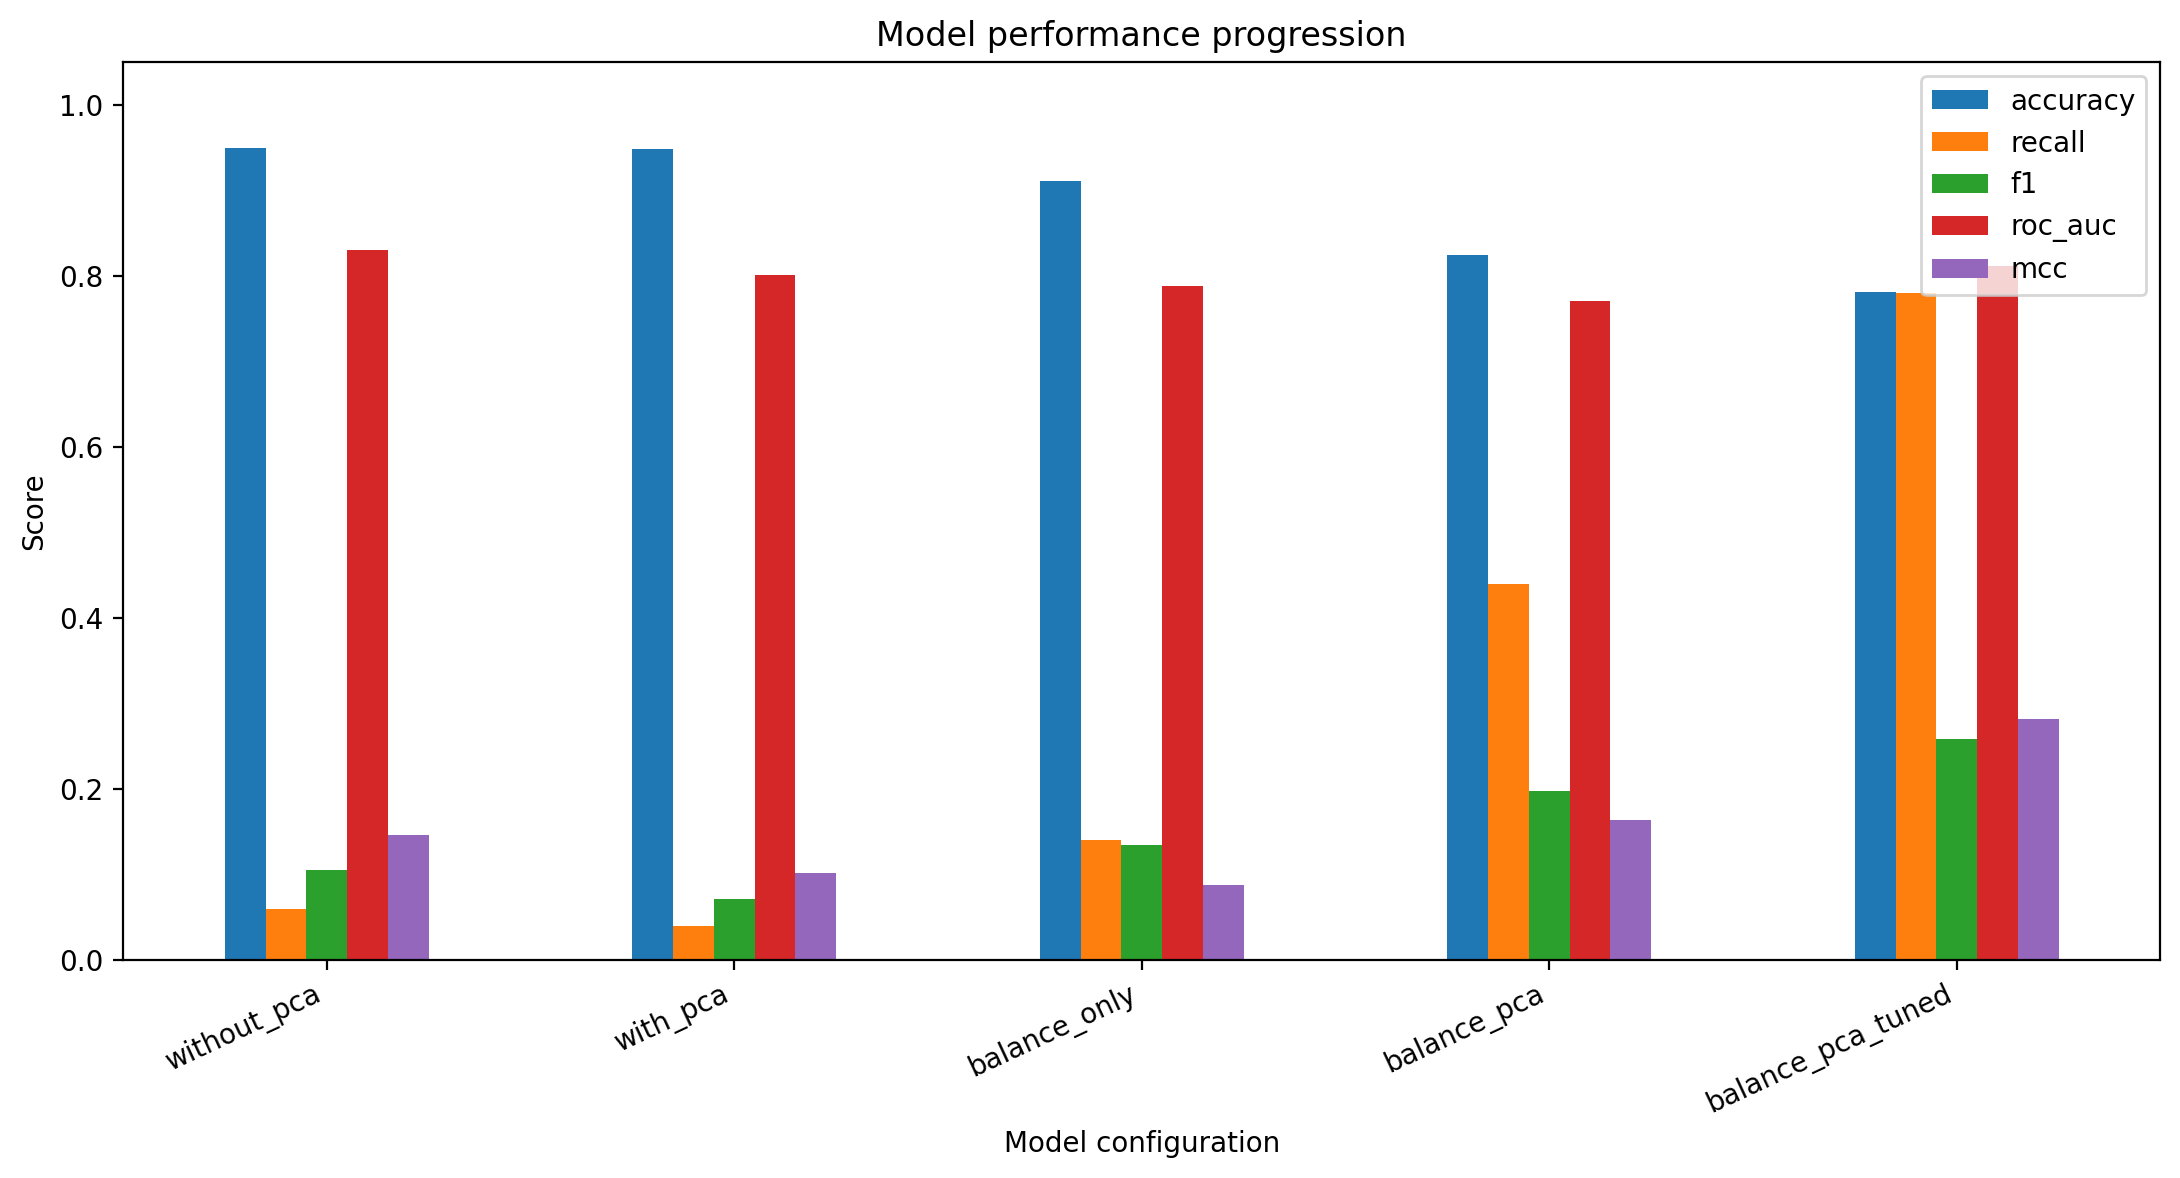
\includegraphics[width=0.90\textwidth]{../results/final_reproduction/dataset1_model_progression.png}
    \caption{Diễn biến hiệu năng qua các bước tái dựng pipeline trên Dataset 1.}
    \label{fig:d1_model_progression}
\end{figure}

\begin{figure}[H]
    \centering
    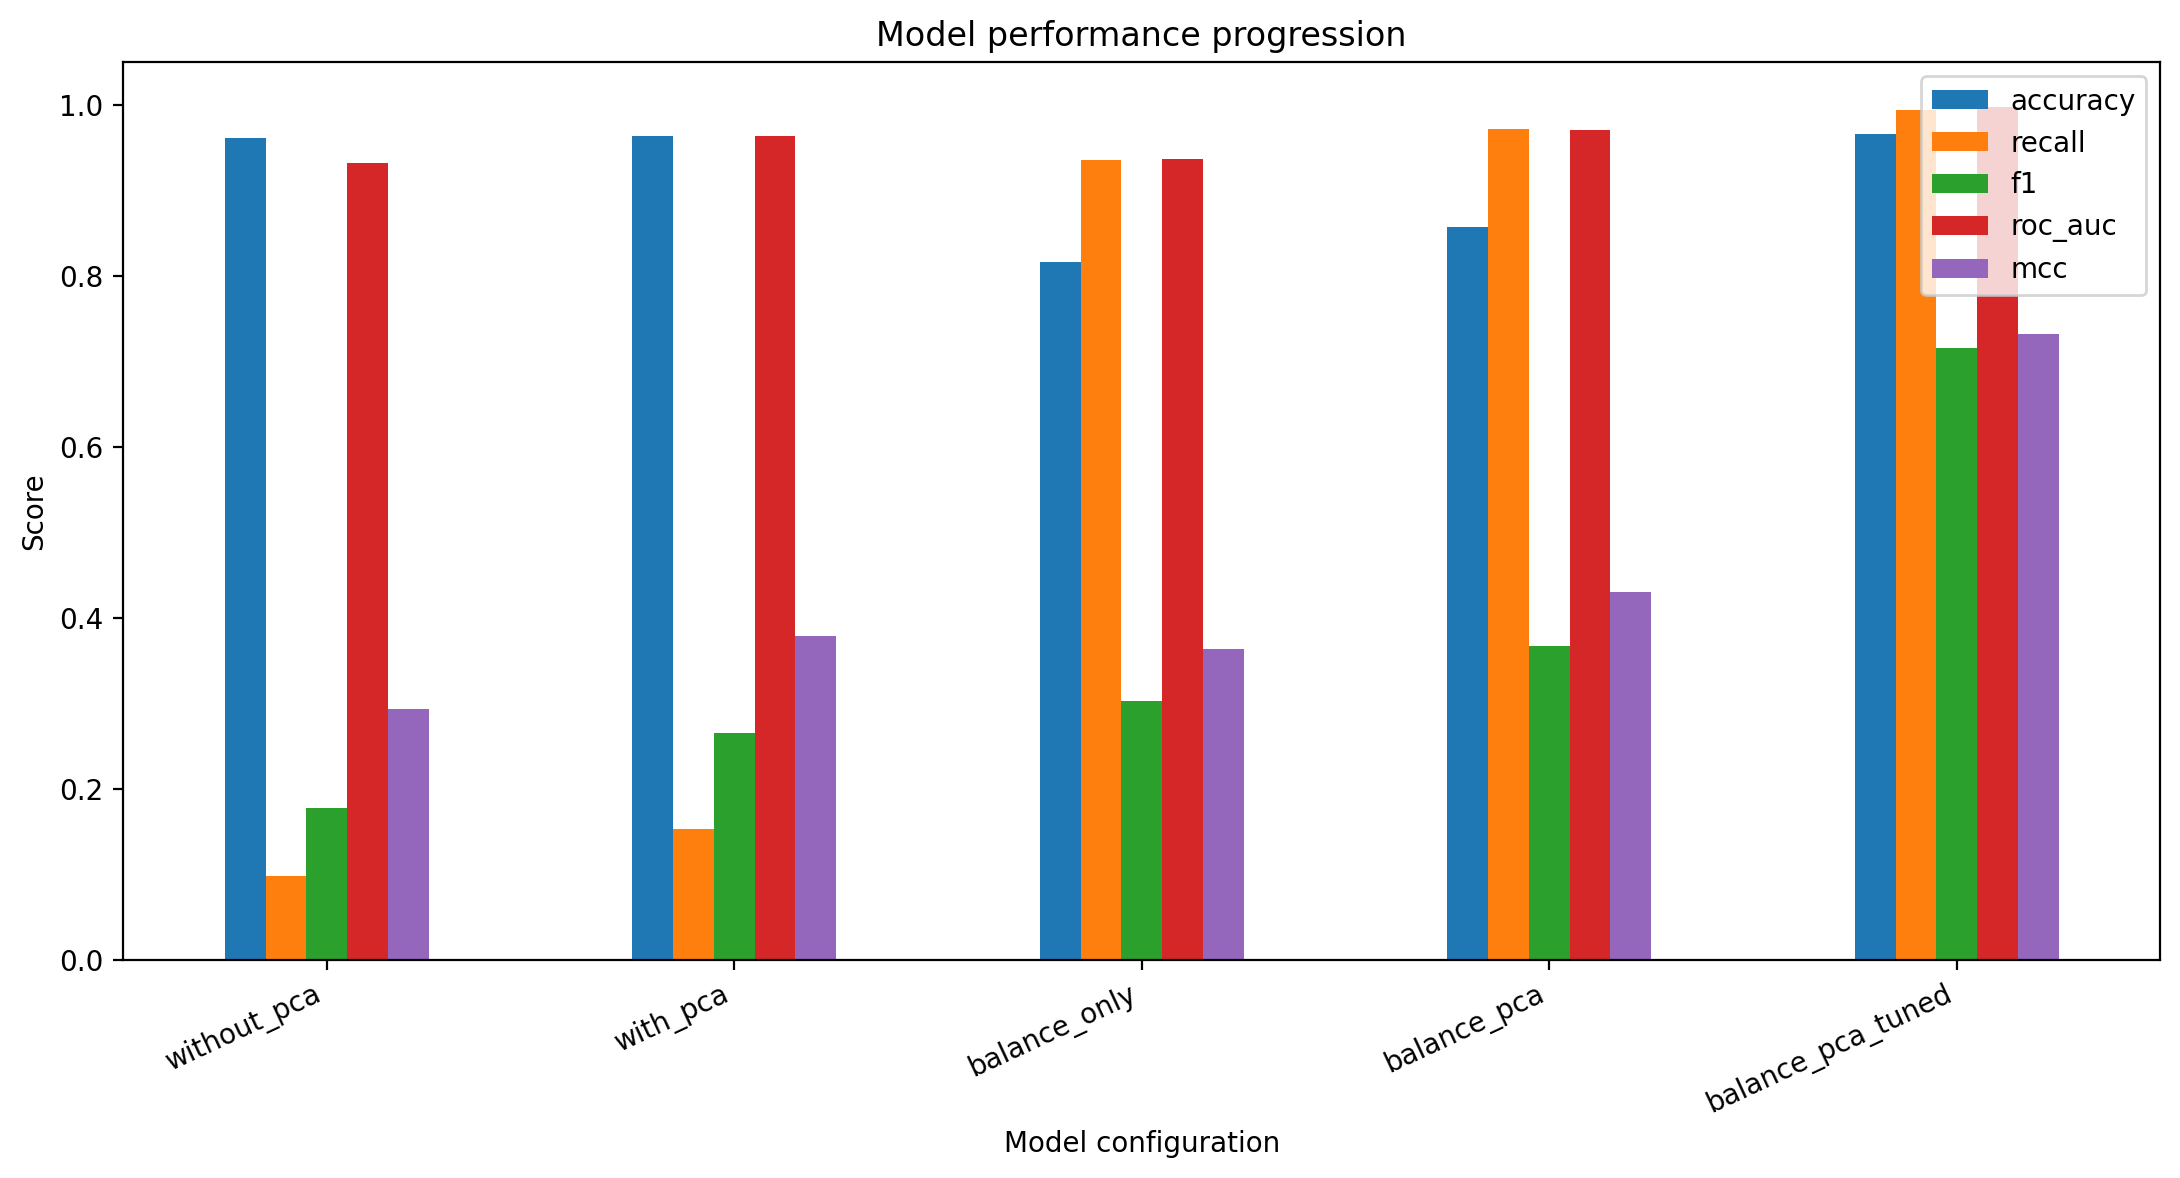
\includegraphics[width=0.90\textwidth]{../results/final_reproduction/dataset2_model_progression.png}
    \caption{Diễn biến hiệu năng qua các bước tái dựng pipeline trên Dataset 2.}
    \label{fig:d2_model_progression}
\end{figure}

Hai hình trên được trình bày riêng cho từng bộ dữ liệu. Nhóm không gộp các metric của Dataset 1 và Dataset 2 vào cùng một hình vì hai bộ dữ liệu khác nhau đáng kể về quy mô, nguồn dữ liệu và độ khó dự đoán.

\section{Kết quả tái hiện so với bài báo}

Sau khi hoàn thiện pipeline theo cách hiểu từ bài báo, Dataset 1 sử dụng SMOTE và giữ 11 thành phần PCA, giải thích khoảng 96,50\% phương sai. Dataset 2 sử dụng Random UnderSampler và giữ 11 thành phần PCA, giải thích khoảng 95,86\% phương sai. Bảng~\ref{tab:reproduction_comparison} chỉ đối chiếu các chỉ số có giá trị tương ứng được bài báo công bố.

\begin{table}[H]
\centering
\caption{Đối chiếu kết quả công bố và kết quả tái hiện}
\label{tab:reproduction_comparison}
\begin{tabular}{llrrr}
\toprule
\textbf{Dữ liệu} & \textbf{Chỉ số} & \textbf{Bài báo} & \textbf{Tái hiện} & \textbf{Chênh lệch}\\
\midrule
Dataset 1 & CV Accuracy & 0,9532 & 0,7652 & -0,1880\\
Dataset 2 & CV Accuracy & 0,9903 & 0,9654 & -0,0249\\
Dataset 2 & MCC & 0,9634 & 0,7322 & -0,2312\\
Dataset 2 & Cohen's Kappa & 0,9632 & 0,6993 & -0,2639\\
\bottomrule
\end{tabular}
\end{table}

Dataset 2 tái hiện gần kết quả công bố hơn về Accuracy, nhưng MCC và Cohen's Kappa vẫn thấp hơn đáng kể. Dataset 1 còn sai khác lớn. Do đó, nhóm không tuyên bố đã tái lập hoàn toàn các con số của tác giả. Một số chi tiết triển khai như thời điểm resampling, cách chia dữ liệu, encoding, random seed, hyperparameter và cách tổng hợp chỉ số cross-validation có thể tạo ra sai khác.

Quan trọng hơn, bài báo không cung cấp một bộ kết quả tương ứng trên tập test giữ nguyên phân bố lớp để nhóm đối chiếu trực tiếp với phần đánh giá bổ sung của mình. Vì vậy, các kết quả trên test giữ nguyên phân bố lớp trong phần sau chỉ được dùng để so sánh \textbf{các cấu hình của nhóm với nhau trên cùng một giao thức}.

\section{Ablation: vai trò của balancing, PCA và tuning}

Kết quả ở Bảng~\ref{tab:model_progression} cho phép rút ra ba nhận xét. Thứ nhất, Accuracy đơn lẻ không phù hợp để lựa chọn mô hình trong bài toán mất cân bằng: baseline Dataset 1 có Accuracy 0,9501 nhưng bỏ sót gần như toàn bộ ca đột quỵ. Thứ hai, PCA không phải lúc nào cũng cải thiện mô hình nếu đứng riêng lẻ; trên Dataset 1, thêm PCA vào baseline làm Recall giảm từ 0,06 xuống 0,04. Thứ ba, tác động lớn nhất xuất hiện khi balancing được kết hợp với PCA và tuning, đặc biệt ở Recall, F1 và MCC.

Do đó, trong phần còn lại của chương, SMOTE trên Dataset 1 và Random UnderSampler trên Dataset 2 được xem là \textbf{baseline xử lý mất cân bằng theo pipeline tái hiện}, không được gọi là đề xuất mới. Thử nghiệm có/không PCA được xem là ablation. Những phương pháp thay thế balancing hoặc thay đổi quy tắc quyết định mới được xem là hướng mở rộng của nhóm.

\section{Mở rộng phương pháp xử lý mất cân bằng}

Để so sánh công bằng, nhóm chia train/test trước khi ước lượng các tham số tiền xử lý. Imputation, chuẩn hóa, encoding, PCA và resampling chỉ được fit trên dữ liệu huấn luyện hoặc bên trong từng fold. Tập test giữ nguyên phân bố lớp và không được resample. Ngưỡng phân loại được lựa chọn từ validation hoặc dự đoán out-of-fold rồi khóa trước khi đánh giá test.

\subsection{Dataset 1: từ SMOTE sang SMOTENC và cost-sensitive learning}

SMOTE là phương pháp thuộc baseline tái hiện của Dataset 1. Nhóm mở rộng bằng hai hướng: \textbf{SMOTENC}, nhằm xử lý phù hợp hơn các biến phân loại, và \textbf{cost-sensitive XGBoost} thông qua trọng số lớp, tránh tạo thêm quan sát tổng hợp. Mỗi phương pháp được khảo sát cả có và không PCA.

\begin{table}[H]
\centering
\scriptsize
\caption{Dataset 1: một số cấu hình tại ngưỡng mặc định 0,5 trên cùng tập test giữ nguyên phân bố lớp}
\label{tab:d1_methods_default}
\resizebox{\linewidth}{!}{%
\begin{tabular}{llrrrrrr}
\toprule
\textbf{Phương pháp} & \textbf{PCA} & \textbf{Accuracy} & \textbf{Precision} & \textbf{Recall} & \textbf{F1} & \textbf{ROC-AUC} & \textbf{MCC}\\
\midrule
SMOTE & Không & 0,8620 & 0,1946 & 0,5800 & 0,2915 & 0,8412 & 0,2791\\
SMOTE & Có & 0,8513 & 0,1964 & 0,6600 & 0,3028 & 0,8195 & 0,3033\\
SMOTENC & Không & 0,9295 & 0,2963 & 0,3200 & 0,3077 & 0,8290 & 0,2709\\
SMOTENC & Có & 0,9315 & 0,2619 & 0,2200 & 0,2391 & 0,8170 & 0,2044\\
Weighted & Không & 0,9511 & 0,5000 & 0,0200 & 0,0385 & 0,8263 & 0,0926\\
Weighted & Có & 0,7329 & 0,1296 & 0,7800 & 0,2222 & 0,8241 & 0,2416\\
\bottomrule
\end{tabular}}
\end{table}

Bảng trên cho thấy không có một phương pháp thống trị mọi metric. SMOTENC không PCA cho F1 cao nhất tại ngưỡng 0,5, nhưng Recall chỉ 0,32. Weighted + PCA giữ Recall 0,78 nhưng Precision thấp. Điều này dẫn đến bước mở rộng thứ hai: tối ưu threshold theo mức Specificity mong muốn.

\begin{table}[H]
\centering
\small
\caption{Dataset 1: các cấu hình được chọn theo Specificity mục tiêu}
\label{tab:improvement_d1}
\resizebox{\linewidth}{!}{%
\begin{tabular}{p{2.1cm} p{4.0cm} r r r r r r}
\toprule
\textbf{Spec. mục tiêu} & \textbf{Cấu hình} & \textbf{Ngưỡng} & \textbf{Precision} & \textbf{Recall} & \textbf{Specificity} & \textbf{F1} & \textbf{MCC}\\
\midrule
85\% & Weighted + PCA & 0,6704 & 0,1944 & 0,7000 & 0,8508 & 0,3043 & 0,3119\\
90\% & Weighted, không PCA & 0,1305 & 0,1870 & 0,4600 & 0,8971 & 0,2659 & 0,2368\\
95\% & Weighted, không PCA & 0,1902 & 0,2381 & 0,3000 & 0,9506 & 0,2655 & 0,2248\\
\bottomrule
\end{tabular}}
\end{table}

Ở mức Specificity khoảng 85\%, Weighted + PCA đạt Recall 0,70, F1 0,3043 và MCC 0,3119. So với pipeline tái hiện cuối cùng trên cùng test (Recall 0,78; F1 0,2591; MCC 0,2816), phương án này giảm một phần Recall nhưng tăng F1 và MCC, thể hiện sự cân bằng tốt hơn giữa phát hiện ca bệnh và false positive. Đây là \textbf{cải tiến theo tiêu chí cân bằng hiệu năng}, không phải cải thiện đồng thời mọi chỉ số.

\subsection{Dataset 2: Undersampling và cost-sensitive learning}

Random UnderSampler thuộc baseline tái hiện của Dataset 2. Do đó, việc tiếp tục sử dụng undersampling không được xem là một phương pháp mới; nó đóng vai trò mốc so sánh với weighted XGBoost và với các lựa chọn PCA/threshold.

\begin{table}[H]
\centering
\scriptsize
\caption{Dataset 2: so sánh các phương pháp tại ngưỡng mặc định 0,5}
\label{tab:d2_methods_default}
\resizebox{\linewidth}{!}{%
\begin{tabular}{llrrrrrr}
\toprule
\textbf{Phương pháp} & \textbf{PCA} & \textbf{Accuracy} & \textbf{Precision} & \textbf{Recall} & \textbf{F1} & \textbf{ROC-AUC} & \textbf{MCC}\\
\midrule
Undersampling & Không & 0,9799 & 0,7049 & 0,9086 & 0,7939 & 0,9945 & 0,7905\\
Undersampling & Có & 0,9847 & 0,7401 & 0,9886 & 0,8465 & 0,9987 & 0,8484\\
Weighted & Không & 0,9729 & 0,6150 & 0,9726 & 0,7536 & 0,9963 & 0,7618\\
Weighted & Có & 0,9421 & 0,4233 & 0,9932 & 0,5936 & 0,9956 & 0,6282\\
\bottomrule
\end{tabular}}
\end{table}

Trên Dataset 2, Undersampling + PCA vẫn là cấu hình mạnh nhất trong nhóm phương án khảo sát tại threshold 0,5. So với baseline tái hiện cuối cùng trên cùng test, cấu hình được tuning lại trong thực nghiệm mở rộng làm Accuracy tăng từ 0,9664 lên 0,9847, Precision từ 0,5590 lên 0,7401, F1 từ 0,7157 lên 0,8465 và MCC từ 0,7322 lên 0,8484; Recall chỉ giảm từ 0,9944 xuống 0,9886. Như vậy, ở Dataset 2, cải thiện hiện tại chủ yếu đến từ \textbf{quy trình lựa chọn cấu hình/tuning tốt hơn trên cùng họ phương pháp}, chứ chưa phải một thuật toán balancing mới vượt Random UnderSampler.

\begin{table}[H]
\centering
\scriptsize
\caption{Dataset 2: Undersampling + PCA tại các ngưỡng vận hành}
\label{tab:improvement_d2}
\resizebox{\linewidth}{!}{%
\begin{tabular}{lrrrrrrr}
\toprule
\textbf{Chính sách} & \textbf{Accuracy} & \textbf{Precision} & \textbf{Recall} & \textbf{Specificity} & \textbf{F1} & \textbf{AUC} & \textbf{MCC}\\
\midrule
Threshold 0,5 & 0,9847 & 0,7401 & 0,9886 & 0,9846 & 0,8465 & 0,9987 & 0,8484\\
Spec. 85\% & 0,8611 & 0,2346 & 1,0000 & 0,8550 & 0,3801 & 0,9987 & 0,4479\\
Spec. 90\% & 0,9122 & 0,3265 & 0,9998 & 0,9083 & 0,4922 & 0,9987 & 0,5445\\
Spec. 95\% & 0,9518 & 0,4690 & 0,9984 & 0,9497 & 0,6383 & 0,9987 & 0,6668\\
\bottomrule
\end{tabular}}
\end{table}

Recall bằng 1,0000 tại mục tiêu Specificity 85\% không đồng nghĩa dự đoán hoàn hảo. Ngưỡng 0,0462 khiến mô hình phát hiện toàn bộ 47.192 ca dương tính nhưng đồng thời tạo 153.928 false positive; Precision vì vậy chỉ đạt 0,2346. Threshold được xem là tham số vận hành, cần lựa chọn theo chi phí bỏ sót và chi phí báo động giả.

\section{Tổng hợp kết quả và phạm vi của cải tiến}

\begin{table}[H]
\centering
\small
\caption{Kết luận theo từng tầng thực nghiệm}
\label{tab:three_levels_summary}
\resizebox{\linewidth}{!}{%
\begin{tabular}{p{3.1cm} p{4.0cm} p{7.0cm}}
\toprule
\textbf{Tầng} & \textbf{Thực nghiệm} & \textbf{Kết luận}\\
\midrule
Tái hiện tác giả & SMOTE/Undersampling + PCA + XGBoost & Dataset 2 gần paper hơn về Accuracy; Dataset 1 còn sai khác lớn. Chưa tái lập hoàn toàn kết quả công bố.\\
Ablation & Có/không balancing; có/không PCA; trước/sau tuning & Balancing là thành phần quyết định khả năng phát hiện lớp dương tính; PCA có tác động phụ thuộc dataset; tuning cải thiện rõ F1/MCC.\\
Mở rộng Dataset 1 & SMOTENC; Weighted; threshold & Có thể cải thiện F1/MCC hoặc điều khiển trade-off Recall--Specificity, nhưng chưa có cấu hình thống trị mọi metric.\\
Mở rộng Dataset 2 & Weighted; PCA/no-PCA; threshold; tuning lại undersampling & Weighted không vượt Undersampling + PCA. Cấu hình undersampling được tuning lại cải thiện mạnh F1/MCC trên cùng test.\\
\bottomrule
\end{tabular}}
\end{table}

Như vậy, kết quả hiện tại cho phép kết luận rằng nhóm đã \textbf{cải thiện pipeline tái hiện của chính mình} trên một số tiêu chí và đã mở rộng việc xử lý mất cân bằng so với cấu hình gốc. Tuy nhiên, chưa nên phát biểu rằng phương pháp đề xuất đã ``vượt tác giả'', vì bài báo không cung cấp đầy đủ kết quả trên cùng tập test giữ nguyên phân bố lớp và cùng giao thức đánh giá để thực hiện phép so sánh đó.

\section{Giới hạn và hướng cải tiến thuật toán tiếp theo}

Dataset 1 có quy mô nhỏ và số ca đột quỵ ít nên các chỉ số nhạy với cách chia dữ liệu. Dataset 2 là dữ liệu synthetic; do đó, hiệu năng rất cao cần được xác nhận trên dữ liệu thực độc lập. Ngoài ra, các mở rộng hiện tại chủ yếu vẫn nằm ở tầng xử lý mất cân bằng, PCA, tuning và threshold.

Vì vậy, vòng nghiên cứu tiếp theo sẽ giữ cố định split và protocol đã xác lập trong chương này rồi khảo sát một cải tiến ở \textbf{mức thuật toán hoặc hàm mất mát}. Mục tiêu là nâng F1/MCC và giảm false positive mà không đánh đổi quá nhiều Recall. Việc giữ nguyên protocol cho phép xác định liệu cải tiến tiếp theo thực sự đến từ phương pháp mới hay chỉ từ thay đổi cách đánh giá.

\section{Thử nghiệm mở rộng với các mô hình và cơ chế học cho dữ liệu mất cân bằng}

Sau các thử nghiệm tái hiện và cải tiến dựa trên XGBoost, nhóm tiếp tục khảo sát khả năng cải thiện bằng cách thay đổi họ thuật toán và cơ chế xử lý mất cân bằng. Mục tiêu không chỉ là tăng Accuracy, mà ưu tiên khả năng phát hiện lớp \textit{stroke} trong khi hạn chế cảnh báo dương tính giả. Các phương pháp được khảo sát gồm CatBoost, LightGBM, Balanced Random Forest, EasyEnsemble và XGBoost với Focal Loss. Đây là ba hướng mở rộng khác nhau: thay đổi họ boosting, xử lý mất cân bằng ở cấp độ thuật toán và sử dụng ensemble/hàm mất mát chuyên biệt cho lớp thiểu số.

\subsection{Giao thức thực nghiệm mở rộng}

Outer train/test split tiếp tục được giữ cố định ở tỷ lệ 80/20 với \texttt{random\_state=42}. Test set giữ nguyên phân bố ban đầu, không được resample và không tham gia lựa chọn mô hình hay threshold. Từ outer-training set, nhóm tách inner validation với seed 2026 để xác định operating threshold; một điểm vận hành chính yêu cầu Specificity trên validation đạt tối thiểu 85\%. Threshold sau đó được cố định trước khi đánh giá trên outer test.

Các chỉ số báo cáo gồm Accuracy, Precision, Recall, F1, MCC và ROC-AUC. Trong bối cảnh mất cân bằng, F1 và MCC được dùng để đánh giá sự cân bằng tổng thể, còn Recall được xem là guardrail cho khả năng phát hiện stroke. Việc chọn threshold trên validation thay vì hậu nghiệm trên test nhằm hạn chế thiên lệch do lựa chọn điểm vận hành sau khi đã quan sát kết quả cuối.

\subsection{Dataset 1: so sánh các họ mô hình mới}

CatBoost được huấn luyện trực tiếp trên các biến phân loại nguyên bản với \texttt{auto\_class\_weights=Balanced}, không One-Hot Encoding, PCA hay SMOTE. LightGBM giữ toàn bộ training set và dùng \texttt{scale\_pos\_weight}. Balanced Random Forest tạo các mẫu cân bằng bên trong quá trình xây dựng cây. EasyEnsemble và Focal-loss XGBoost được dùng như các thí nghiệm sàng lọc bổ sung cho bài toán mất cân bằng.

\begin{table}[H]
\centering
\scriptsize
\caption{Dataset 1: kết quả các phương pháp mở rộng trên cùng outer test}
\label{tab:d1_new_methods}
\resizebox{\linewidth}{!}{%
\begin{tabular}{lrrrrrrp{3.6cm}}
\toprule
\textbf{Phương pháp} & \textbf{Acc.} & \textbf{Prec.} & \textbf{Recall} & \textbf{F1} & \textbf{MCC} & \textbf{ROC-AUC} & \textbf{Vai trò}\\
\midrule
XGBoost cải tiến (Exp. 13) & 0,8434 & 0,1944 & 0,7000 & 0,3043 & 0,3119 & 0,8241 & Mốc cải tiến trước đó\\
CatBoost & 0,7867 & 0,1640 & \textbf{0,8200} & 0,2733 & 0,3036 & \textbf{0,8364} & Recall/ROC-AUC cao\\
LightGBM weighted & 0,8327 & 0,1543 & 0,5400 & 0,2400 & 0,2220 & 0,7865 & Không cải thiện\\
\textbf{Balanced Random Forest} & \textbf{0,8483} & \textbf{0,2000} & 0,7000 & \textbf{0,3111} & \textbf{0,3184} & 0,8274 & \textbf{Tốt nhất tổng thể}\\
EasyEnsemble$^{*}$ & 0,8454 & 0,1860 & 0,6400 & 0,2883 & 0,2860 & 0,8309 & Screening\\
Focal-loss XGBoost & 0,8405 & 0,1844 & 0,6600 & 0,2882 & 0,2893 & 0,8317 & Không cải thiện\\
\bottomrule
\end{tabular}}
\end{table}

Balanced Random Forest tạo ra điểm vận hành cân bằng nhất. So với XGBoost cải tiến ở Experiment 13, Recall giữ nguyên 0,70, trong khi Accuracy tăng từ 0,8434 lên 0,8483, Precision từ 0,1944 lên 0,2000, F1 từ 0,3043 lên 0,3111 và MCC từ 0,3119 lên 0,3184. Mức tăng tương đối khoảng 2,2\% ở F1 và 2,1\% ở MCC, vì vậy được diễn giải là \textbf{cải thiện biên (marginal improvement)}, không phải sự vượt trội lớn.

CatBoost cho Recall và ROC-AUC cao nhất, lần lượt 0,82 và 0,8364. Điều này cho thấy khả năng xếp hạng nguy cơ tốt khi xử lý trực tiếp biến categorical, nhưng lợi thế ranking chưa chuyển thành F1/MCC tốt nhất tại operating point được chọn. LightGBM, EasyEnsemble và Focal-loss XGBoost không vượt Balanced Random Forest hoặc XGBoost cải tiến trên các chỉ số cân bằng chính.

$^{*}$EasyEnsemble sử dụng cấu hình giới hạn tài nguyên tính toán sau khi cấu hình mặc định không phù hợp với môi trường chạy; vì vậy kết quả được xem là screening experiment, không phải bằng chứng chính để xếp hạng mô hình.

\subsection{Dataset 2: class weighting so với data-level balancing}

Dataset 2 sau làm sạch có 5.542.261 quan sát; outer-training set gồm 4.433.808 và outer-test set gồm 1.108.453 mẫu. LightGBM được chạy trên toàn bộ outer-training set, không undersampling hay SMOTE; mất cân bằng được xử lý bằng \texttt{scale\_pos\_weight}. Kết quả được so sánh với cấu hình XGBoost + undersampling + PCA tốt nhất ở Experiment 13.

\begin{table}[H]
\centering
\scriptsize
\caption{Dataset 2: so sánh XGBoost cải tiến và LightGBM weighted trên full data}
\label{tab:d2_new_methods}
\resizebox{\linewidth}{!}{%
\begin{tabular}{lrrrrrr}
\toprule
\textbf{Phương pháp} & \textbf{Acc.} & \textbf{Prec.} & \textbf{Recall} & \textbf{F1} & \textbf{MCC} & \textbf{ROC-AUC}\\
\midrule
\textbf{XGBoost + undersampling + PCA} & \textbf{0,9847} & \textbf{0,7401} & 0,9886 & \textbf{0,8465} & \textbf{0,8484} & \textbf{0,9987}\\
LightGBM weighted & 0,9587 & 0,5079 & \textbf{0,9926} & 0,6720 & 0,6943 & 0,9973\\
\bottomrule
\end{tabular}}
\end{table}

LightGBM tăng Recall nhẹ từ 0,9886 lên 0,9926 nhưng Precision giảm mạnh từ 0,7401 xuống 0,5079; F1 giảm còn 0,6720 và MCC còn 0,6943. Kết quả cho thấy class weighting giúp hạn chế false negative nhưng tạo nhiều false positive hơn. Trên Dataset 2, \textbf{data-level balancing bằng undersampling kết hợp XGBoost cho trade-off Precision--Recall tốt hơn algorithm-level class weighting của LightGBM}.

CatBoost cũng được khảo sát cho Dataset 2, nhưng huấn luyện full 4,43 triệu quan sát vượt giới hạn bộ nhớ của môi trường thực nghiệm. Một probe dùng stratified subset được thực hiện để kiểm tra tính khả thi, song không được đưa vào bảng so sánh full-data và không được dùng để kết luận hơn/kém so với XGBoost hay LightGBM. Cách trình bày này tránh đánh đồng một thí nghiệm giới hạn tài nguyên với các experiment sử dụng toàn bộ training set.

\subsection{Đúc kết từ thử nghiệm mở rộng}

Các thử nghiệm cho thấy thay thế XGBoost bằng một họ thuật toán mới không tự động tạo ra cải thiện. Với Dataset 1 nhỏ và mất cân bằng mạnh, Balanced Random Forest cho cải thiện nhỏ nhưng nhất quán về Accuracy, Precision, F1 và MCC khi giữ nguyên Recall. CatBoost lại nổi bật ở Recall và ROC-AUC, cho thấy một operating objective khác có thể dẫn đến lựa chọn mô hình khác.

Với Dataset 2 quy mô lớn, XGBoost kết hợp undersampling và PCA vẫn là cấu hình tốt nhất xét đồng thời Precision, Recall, F1 và MCC. LightGBM weighted đạt Recall cao hơn nhưng phải đánh đổi bằng số false positive lớn hơn. Do đó, ảnh hưởng của \textbf{cơ chế xử lý mất cân bằng và operating threshold ít nhất quan trọng tương đương việc lựa chọn họ mô hình}.

Kết luận của giai đoạn mở rộng không phải là một thuật toán mới có thể thay thế XGBoost trong mọi trường hợp. Thay vào đó, phương pháp tối ưu phụ thuộc vào cấu trúc và quy mô dữ liệu: \textbf{Balanced Random Forest là phương án mở rộng tốt nhất cho Dataset 1}, trong khi \textbf{XGBoost + undersampling + PCA tiếp tục là cấu hình tốt nhất cho Dataset 2}. Các kết quả âm tính của LightGBM, EasyEnsemble và Focal-loss XGBoost cũng được giữ lại để bảo đảm báo cáo phản ánh đầy đủ quá trình thử nghiệm thay vì chỉ lựa chọn hậu nghiệm các kết quả thuận lợi.

% Trigger CI rebuild after adding the PDF workflow.

\FloatBarrier
\clearpage
\chapter*{KẾT LUẬN}
\addcontentsline{toc}{chapter}{KẾT LUẬN}

Báo cáo đã giúp chúng tôi hiểu rõ quy trình xây dựng mô hình dự đoán
và áp dụng một số kỹ thuật tối ưu, bao gồm tiền xử lý dữ liệu, xử lý mất cân
bằng bằng SMOTE hoặc undersampling, giảm chiều bằng PCA và huấn luyện
mô hình XGBoost. Qua đó, chúng tôi nhận thấy Accuracy không đủ để đánh
giá mô hình trong bài toán mất cân bằng; Recall, F1-score, MCC và
ROC-AUC cần được xem xét đồng thời.

Quá trình tái hiện cũng cho thấy bài báo gốc chưa mô tả đầy đủ thứ tự
chia dữ liệu, resampling, PCA và các tham số thực nghiệm. Vì vậy,
chúng tôi xây dựng một protocol minh bạch hơn: chia train/test trước,
chỉ thực hiện preprocessing và balancing trên tập huấn luyện, đồng thời
giữ nguyên phân bố lớp của tập test để tránh rò rỉ dữ liệu.

Kết quả cải thiện cho thấy việc kết hợp balancing, PCA, tuning và lựa
chọn operating threshold giúp tăng đáng kể khả năng phát hiện lớp
stroke. Trên Dataset 1, Balanced Random Forest tạo ra cải thiện nhẹ về
F1-score và MCC so với cấu hình XGBoost có trọng số. Trên Dataset 2,
XGBoost kết hợp undersampling và PCA vẫn cho sự cân bằng tốt nhất giữa
Precision, Recall, F1-score và MCC; LightGBM đạt Recall cao nhưng
Precision thấp hơn.

Từ các thí nghiệm, chúng tôi rút ra rằng không có một mô hình duy nhất
tốt nhất trên mọi bộ dữ liệu. Hiệu quả dự đoán phụ thuộc không chỉ vào
thuật toán mà còn vào protocol đánh giá, phương pháp xử lý mất cân bằng
và ngưỡng quyết định. Đây là những điểm cải thiện chính được rút ra từ
việc tái hiện và mở rộng bài báo gốc.
\FloatBarrier
\clearpage

% ==================== TÀI LIỆU THAM KHẢO ====================
\chapter*{TÀI LIỆU THAM KHẢO}
\addcontentsline{toc}{chapter}{TÀI LIỆU THAM KHẢO}
\begin{enumerate}[label={[\arabic*]},leftmargin=1.2cm]
\item \hypertarget{bib:1}{}Dev S, Wang H, Nwosu CS, Jain N, Veeravalli B, John D. A predictive analytics approach for stroke prediction using machine learning and neural networks. \textit{Healthc Anal.} 2022;2:100032. \url{https://doi.org/10.1016/j.health.2022.100032}.
\item \hypertarget{bib:2}{}Bikku T, Fritz RA, Colón YJ, Herrera F. Machine learning identification of organic compounds using visible light. 2022. \url{https://doi.org/10.48550/ARXIV.2204.11832}.
\item \hypertarget{bib:3}{}Kovtun O, Kovtun V. Machine Learning-Based Approach to Transcribing Language Units. In: 2024 14th International Conference on Advanced Computer Information Technologies (ACIT), Ceske Budejovice. Czech Republic: IEEE; 2024. pp. 636--639. \url{https://doi.org/10.1109/ACIT62333.2024.10712598}.
\item \hypertarget{bib:4}{}Gupta A et al. Predicting stroke risk: an effective stroke prediction model based on neural networks. \textit{J Neurorestoratol.} 2024:100156. \url{https://doi.org/10.1016/j.jnrt.2024.100156}.
\item \hypertarget{bib:5}{}JalajaJayalakshmi V, Geetha V, Ijaz MM. Analysis and Prediction of Stroke using Machine Learning Algorithms. In: 2021 International Conference on Advancements in Electrical, Electronics, Communication, Computing and Automation (ICAECA), Coimbatore. India: IEEE; 2021. pp. 1--5. \url{https://doi.org/10.1109/ICAECA52838.2021.9675545}.
\item \hypertarget{bib:6}{}Bikku T. Multi-layered deep learning perceptron approach for health risk prediction. \textit{J Big Data.} 2020;7(1):50. \url{https://doi.org/10.1186/s40537-020-00316-7}.
\item \hypertarget{bib:7}{}Upadhyay R, Panse P, Soni A, Rathore Bhatt U. Principal component analysis as a dimensionality reduction and data preprocessing technique. \textit{SSRN Electron J.} 2019. \url{https://doi.org/10.2139/ssrn.3364221}.
\item \hypertarget{bib:8}{}Izonin I, Gamra A, Boychuk O, et al. PCA-NuSVR Framework for Predicting Local and Global Indicators of Tunneling-induced Building Damage. Proceedings of the 1st International Conference on Smart Automation \& Robotics for Future Industry (SMARTINDUSTRY 2024). 2024;3699:32--46.
\item \hypertarget{bib:9}{}Booker NK, Knights P, Gates JD, Clegg RE. Applying principal component analysis (PCA) to the selection of forensic analysis methodologies. \textit{Eng Fail Anal.} 2022;132:105937. \url{https://doi.org/10.1016/j.engfailanal.2021.105937}.
\item \hypertarget{bib:10}{}Mochurad L, Panto R. A Parallel Algorithm for the Detection of Eye Disease. In: Advances in Intelligent Systems, Computer Science and Digital Economics IV, vol. 158. Hu Z, Wang Y, He M, eds. Lecture Notes on Data Engineering and Communications Technologies. Cham: Springer Nature Switzerland; 2023. pp. 111--125. \url{https://doi.org/10.1007/978-3-031-24475-9_10}.
\item \hypertarget{bib:11}{}Althiban AS, Alharbi HM, Al Khuzayem LA, Eassa FE. Predicting software defects in hybrid MPI and OpenMP parallel programs using machine learning. \textit{Electronics.} 2023;13(1):182. \url{https://doi.org/10.3390/electronics13010182}.
\item \hypertarget{bib:12}{}Mochurad L, Kotsiumbas O, Protsyk I. A model for weather forecasting based on parallel calculations. In: Advances in Artificial Systems for Medicine and Education VI, vol. 159. Hu Z, Ye Z, He M, eds. Lecture Notes on Data Engineering and Communications Technologies. Cham: Springer Nature Switzerland; 2023. pp. 35--46. \url{https://doi.org/10.1007/978-3-031-24468-1_4}.
\item \hypertarget{bib:13}{}Ali S, et al. Explainable Artificial Intelligence (XAI): What we know and what is left to attain Trustworthy Artificial Intelligence. \textit{Inf Fusion.} 2023;99:101805. \url{https://doi.org/10.1016/j.inffus.2023.101805}.
\item \hypertarget{bib:14}{}Bikku T. Fuzzy associated trust-based data security in cloud computing by mining user behaviour. \textit{Int J Adv Intell Paradig.} 2023;25(3/4):382--97. \url{https://doi.org/10.1504/IJAIP.2023.132377}.
\item \hypertarget{bib:15}{}Tazin T, Alam MN, Dola NN, Bari MS, Bourouis S, Monirujjaman Khan M. Stroke disease detection and prediction using robust learning approaches. \textit{J Healthc Eng.} 2021:1--12. \url{https://doi.org/10.1155/2021/7633381}.
\item \hypertarget{bib:16}{}Patereha Y, Melnyk M. Prediction of the occurrence of stroke based on machine learning models. \textit{Comput Des Syst Theory Pract.} 2024;6(1):17--27. \url{https://doi.org/10.23939/cds2024.01.017}.
\item \hypertarget{bib:17}{}Dritsas E, Trigka M. Stroke risk prediction with machine learning techniques. \textit{Sensors.} 2022;22(13):4670. \url{https://doi.org/10.3390/s22134670}.
\item \hypertarget{bib:18}{}Sailasya G, Kumari GL. Analyzing the performance of stroke prediction using ML classification algorithms. \textit{Int J Adv Comput Sci Appl.} 2021;12(6). \url{https://doi.org/10.14569/IJACSA.2021.0120662}.
\item \hypertarget{bib:19}{}Dhillon S, Bansal C, Sidhu B. Machine learning based approach using xgboost for heart stroke prediction. International Conference on Emerging Technologies: AI, IoT, and CPS for Science \& Technology Applications. 2021. p. 1--6.
\item \hypertarget{bib:20}{}Chung C-C, Su EC-Y, Chen J-H, Chen Y-T, Kuo C-Y. XGBoost-based simple three-item model accurately predicts outcomes of acute ischemic stroke. \textit{Diagnostics.} 2023;13(5):842. \url{https://doi.org/10.3390/diagnostics13050842}.
\item \hypertarget{bib:21}{}Tumpanjawat. Stroke Prediction: EDA | Resampling | XGBoost. Kaggle. 2024. Available: \url{https://www.kaggle.com/code/tumpanjawat/stroke-prediction-eda-resampling-xgboost}.
\item \hypertarget{bib:22}{}Mainali S, Darsie ME, Smetana KS. Machine learning in action: stroke diagnosis and outcome prediction. \textit{Front Neurol.} 2021;12:734345. \url{https://doi.org/10.3389/fneur.2021.734345}.
\item \hypertarget{bib:23}{}Fang G, Huang Z, Wang Z. Predicting ischemic stroke outcome using deep learning approaches. \textit{Front Genet.} 2022;12:827522. \url{https://doi.org/10.3389/fgene.2021.827522}.
\item \hypertarget{bib:24}{}Srinivasu PN, Sirisha U, Sandeep K, Praveen SP, Maguluri LP, Bikku T. An interpretable approach with explainable ai for heart stroke prediction. \textit{Diagnostics.} 2024;14(2):128. \url{https://doi.org/10.3390/diagnostics14020128}.
\item \hypertarget{bib:25}{}Mienye ID, Jere N. Optimized ensemble learning approach with explainable ai for improved heart disease prediction. \textit{Information.} 2024;15(7):394. \url{https://doi.org/10.3390/info15070394}.
\item \hypertarget{bib:26}{}Singamaneni KK, Budati AK, Bikku T. An Efficient Q-KPABE framework to enhance cloud-based iot security and privacy. \textit{Wirel Pers Commun.} 2024. \url{https://doi.org/10.1007/s11277-024-10908-8}.
\item \hypertarget{bib:27}{}Bikku T, Malligunta KK, Thota S, Surapaneni PP. Improved quantum algorithm: a crucial stepping stone in quantum-powered drug discovery. \textit{J Electron Mater.} 2024. \url{https://doi.org/10.1007/s11664-024-11275-7}.
\item \hypertarget{bib:28}{}Da Poian V, et al. Exploratory data analysis (EDA) machine learning approaches for ocean world analog mass spectrometry. \textit{Front Astron Space Sci.} 2023;10:1134141. \url{https://doi.org/10.3389/fspas.2023.1134141}.
\item \hypertarget{bib:29}{}Elreedy D, Atiya AF. A Comprehensive Analysis of Synthetic Minority Oversampling Technique (SMOTE) for handling class imbalance. \textit{Inf Sci.} 2019;505:32--64. \url{https://doi.org/10.1016/j.ins.2019.07.070}.
\item \hypertarget{bib:30}{}Nohara Y, Matsumoto K, Soejima H, Nakashima N. Explanation of machine learning models using shapley additive explanation and application for real data in hospital. \textit{Comput Methods Programs Biomed.} 2022;214:106584. \url{https://doi.org/10.1016/j.cmpb.2021.106584}.
\item \hypertarget{bib:31}{}Soriano F. Stroke Prediction Dataset. 2024. Available: \url{https://www.kaggle.com/datasets/fedesoriano/stroke-prediction-dataset}.
\item \hypertarget{bib:32}{}Pranav Prakash. Stroke Prediction -- Health Care Synthetic Dataset. 2024. Available: \url{https://www.kaggle.com/datasets/pranavp1999/strokeprediction-health-care-synthetic-dataset}.
\item \hypertarget{bib:33}{}Sahriar S, et al. Unlocking stroke prediction: harnessing projection-based statistical feature extraction with ML algorithms. \textit{Heliyon.} 2024;10(5):e27411. \url{https://doi.org/10.1016/j.heliyon.2024.e27411}.
\item \hypertarget{bib:34}{}Wisesty UN, Wirayuda TAB, Sthevanie F, Rismala R. Analysis of data and feature processing on stroke prediction using wide range machine learning model. \textit{J Online Inform.} 2024;9(1):29--40. \url{https://doi.org/10.15575/join.v9i1.1249}.
\item \hypertarget{bib:35}{}Yaqoob A, Verma NK, Aziz RM, Saxena A. Enhancing Feature Selection Through Metaheuristic Hybrid Cuckoo Search and Harris Hawks Optimization for Cancer Classification. In: Metaheuristics for Machine Learning, 1st ed. Kalita K, Ganesh N, Balamurugan S, eds. Wiley; 2024. pp. 95--134. \url{https://doi.org/10.1002/9781394233953.ch4}.
\item \hypertarget{bib:36}{}Abdel-Basset M, Abdel-Fatah L, Sangaiah AK. Metaheuristic algorithms: a comprehensive review. In: Computational Intelligence for Multimedia Big Data on the Cloud with Engineering Applications. Elsevier; 2018. pp. 185--231. \url{https://doi.org/10.1016/B978-0-12-813314-9.00010-4}.
\item \hypertarget{bib:37}{}Yaqoob A, Verma NK, Aziz RM, Shah MA. Optimizing cancer classification: a hybrid RDO-XGBoost approach for feature selection and predictive insights. \textit{Cancer Immunol Immunother.} 2024;73(12):261. \url{https://doi.org/10.1007/s00262-024-03843-x}.
\item \hypertarget{bib:38}{}Yaqoob A, Verma NK, Aziz RM, Shah MA. RNA-Seq analysis for breast cancer detection: a study on paired tissue samples using hybrid optimization and deep learning techniques. \textit{J Cancer Res Clin Oncol.} 2024;150(10):455. \url{https://doi.org/10.1007/s00432-024-05968-z}.
\end{enumerate}


\end{document}
